\section{Graph Algorithms}

  A huge portion of problems can be solved by representing as a \textit{graph} data structure. In here, we will explore various problems that can be solved through \textit{graph algorithms}. 

\subsection{Representations and Properties}

  All graphs consist of a set of vertices/nodes $V$ and edges $E$. This tuple is what makes up a graph. We denote $|V| = n, |E| = m$. 

  \begin{definition}[Undirected Graphs]
    An \textbf{undirected graph} $G(V, E)$ is a tuple, where $V = \{v_1, \ldots, v_n\}$ is the vertex set and $E = \{\{v_i, v_j\}\}$ is the edge set (note that it is a set of sets!). 
    \begin{enumerate}
      \item The \textbf{degree} $d_v$ of a vertex $v$ is the number of edges incident to it. 
      \item A \textbf{path} is a sequence of vertices where adjacent vertices are connected by a path in $E$. It's \textbf{length} is the number of edges in the path. 
      \item A \textbf{cycle/circuit} is a path that has the same start and end. 
      \item A graph is \textbf{connected} if for every pair of vertices $e_i, e_j \in E$, there is a path from $e_i$ to $e_j$. 
      \item A \textbf{connected component} is a maximal subset of connected vertices. 
    \end{enumerate}
  \end{definition}

  \begin{definition}[Directed Graph]
    A \textbf{directed graph} $G(V, E)$ is a tuple, where $V = \{v_1, \ldots, v_n\}$ is the vertex set and $E = \{(v_i, v_j)\}$ is the edge set (note that it is a set of tuples, so $(i, j) \neq ( j, i)$).
    \begin{enumerate}
      \item The \textbf{in/out degree} $d_{v, i}, d_{v, o}$ of a vertex $v$ is the number of edges going in to or out from $v$. 
      \item A \textbf{path} is a sequence of vertices where adjacent vertices are connected by a path in $E$. It's \textbf{length} is the number of edges in the path. 
      \item A \textbf{cycle/circuit} is a path that has the same start and end. 
      \item A directed graph is \textbf{strongly connected} if for every pair of vertices $e_i, e_j \in E$, there is a path from $e_i$ to $e_j$.\footnote{Obviously, a connected undirected graph is also strongly connected.}
      \item A \textbf{strongly connected component} is a maximal subset of connected vertices. 
    \end{enumerate}
  \end{definition}

  In fact, from these definitions alone, we can solve an ancient puzzle called \textit{the Bridges of Konigsberg}. Euler, in trying to solve this problem, had invented graph theory. 

  \begin{example}[Bridges of Konigsberg]
    Is there a way to walk that crosses each bridge \textit{exactly} once? 

    \begin{figure}[H]
      \centering
      \begin{subfigure}[b]{0.48\textwidth}
      \centering
        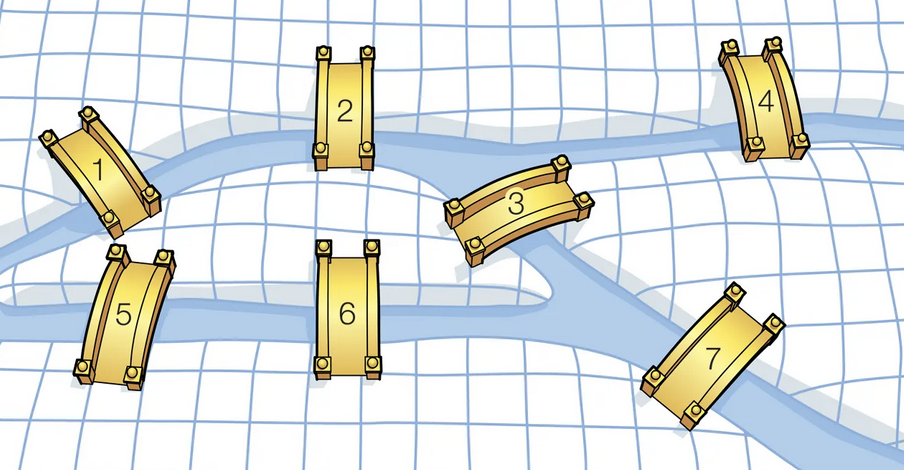
\includegraphics[scale=0.4]{img/bridges.png}
        \caption{Figure of the bridges of Konigsberg.}
        \label{fig:bridges}
      \end{subfigure}
      \hfill 
      \begin{subfigure}[b]{0.48\textwidth}
      \centering
        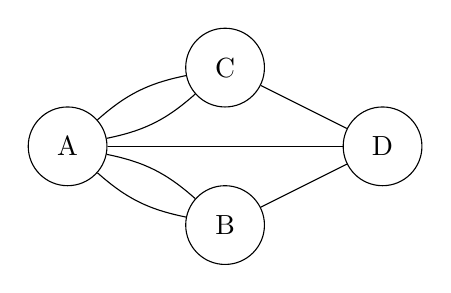
\begin{tikzpicture} 
          \tikzstyle{every node}=[circle, draw, minimum size=1cm]
          
          \node (A) at (0,0) {A};
          \node (B) at (2,-1) {B};
          \node (C) at (2,1) {C};
          \node (D) at (4,0) {D}; 
                
          \draw (A) to[bend left=15] (B);
          \draw (A) to[bend right=15] (B);
          \draw (A) to[bend left=15] (C);
          \draw (A) to[bend right=15] (C);
          \draw (A) -- (D);
          \draw (B) -- (D);
          \draw (C) -- (D);
        \end{tikzpicture}
        \caption{Graph representation. }
        \label{fig:graph_bridges}
      \end{subfigure}
      \caption{It can be decomposed into this undirected graph.}
      \label{fig:konigsberg}
    \end{figure}
     
    Euler's observation is that except for start and end points, a talk leaves any vertex by different edge that the incoming edge. Therefore, the degree (number of edges incident on it) must have an even number, so all but 2 vertices must have an even degree. Since every vertex has an odd degree, there is no way of doing it. 
  \end{example}

  In addition to the \textit{adjacency list} representation, another way in which we represent a directed graph is through \textit{adjacency matrices}. 

  \begin{definition}[Adjacency Matrix]
    In a finite directed graph $(V, E)$, we can construct a bijection from $V$ to the natural numbers and so we label each element in $V$ with $i \in \mathbb{N}$. Then, we can construct a matrix $A$ such that 
    \begin{equation}
      A_{ij} = \begin{cases} 1 & \text{ if } (i, j) \in E \\ 0 & \text{ if } (i, j) \not\in E \end{cases}
    \end{equation}
  \end{definition}

  \begin{example}[Adjacency List vs Matrix]
    Given a graph, we can completely represent it with a list of adjacent vertices for each vertex or an adjacency matrix. 
    \begin{center}
    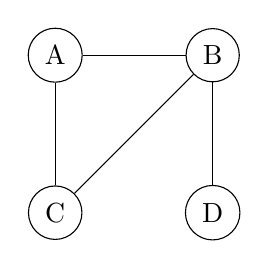
\begin{tikzpicture}
      \node[circle, draw] (C) at (0,0) {C};
      \node[circle, draw] (D) at (2,0) {D};
      \node[circle, draw] (B) at (2,2) {B};
      \node[circle, draw] (A) at (0,2) {A};

      \draw (A) -- (B);
      \draw (B) -- (C);
      \draw (A) -- (C);
      \draw (B) -- (D);
    \end{tikzpicture}
    \end{center}
    An adjacency list would look something like this 
    \[
    \begin{aligned}
    A &: B, C \\
    B &: A, C, D \\
    C &: A, B \\
    D &: B
    \end{aligned}
    \]
    and the adjacency matrix looks like this: 
    \begin{center}
    \begin{tikzpicture}
      \matrix[matrix of math nodes, nodes in empty cells,          column sep=-\pgflinewidth, row sep=-\pgflinewidth,          nodes={minimum size=7mm, anchor=center, outer sep=0pt}] (adjacency) {
        & |(a)| A & |(b)| B & |(c)| C & |(d)| D \\
        |(A)| A & 0 & 1 & 1 & 0 \\
        |(B)| B & 1 & 0 & 1 & 1 \\
        |(C)| C & 1 & 1 & 0 & 0 \\
        |(D)| D & 0 & 1 & 0 & 0 \\
      };
    \end{tikzpicture}
    \end{center}
  \end{example}

  While the adjacency matrix does have its advantages and has a cleaner form, usually in sparse graphs this is memory inefficient due to there being an overwhelming number of $0$s. 

  \begin{definition}[Trees]
    An undirected graph $G(V, E)$ is a \textbf{tree} if 
    \begin{enumerate}
      \item $G$ is connected. 
      \item $G$ has no cycles.\footnote{This makes sense, since to get back to a previous vertex you must backtrack.}
    \end{enumerate}
    Removing the first requirement gives us the definition of a \textbf{forest}, which is a collection of trees. Conversely, if $G(V, E)$ is connected  and $|E| = n - 1$, then $G$ is a tree. 
  \end{definition}

  \begin{theorem}[Properties of Trees]
    If $G(V, E)$ is a tree, then 
    \begin{enumerate}
      \item There exists a $v \in V$ s.t. $d_v = 1$, called a \textbf{leaf node}. 
      \item $|E| = |V| - 1 = n - 1$. 
    \end{enumerate}
  \end{theorem}
  \begin{proof}
    The outlines are quite intuitive. 
    \begin{enumerate}
      \item There must be some leaf node since if there wasn't, then we would have a cycle. We can use proof by contradiction. 
      \item We can use proof by induction. We start off with one vertex and to construct a tree, we must add one edge and one vertex at every step, keeping this invariant.  
    \end{enumerate}
  \end{proof}

\subsection{Exploration}

  Given two $v, s \in V$ either directed or undirected, how can we find the shortest path from $v$ to $s$? We can do with either with DFS or BFS. 

  Now, in order to traverse this graph, we basically want to make an algorithm that starts at a node, prints it value, and then goes to all of its neighbors (which we can access through the adjacency list) to print them out. Thus, this is by nature recursive. We don't want the algorithm to loop around printing nodes infinitely often, so we must create a base case that tells the algorithm to not print out a node. It makes sense to create a set of visited nodes, which we can add to whenever we reach a new node. So, if we ever come onto a node that we have visited, we can just tell the function to do nothing. 

  Though recursion really makes this simple, we can construct an iterative approach that uses stacks. Note that in recursion, we are really making a call stack of different functions. We can be explicit about this by actually implementing a stack, which would store all the nodes that we have discovered, but not yet explored from )i.e. all the current nodes). At each iteration, we would pick a node to continue exploring, and since this is a DFS, we would want to implement a LIFO stack so that the last element we input in is the first thing that we should explore from, i.e. we always explore from the last node discovered. 

  \begin{definition}[DFS]
    The recursive algorithm is 
    \begin{lstlisting}
      visited = set() 
      def dfs(start): 
        if start not in visited: 
          visited.add(start) 
          # do something 
          neighbors = ... 
          for neighbor in neighbors: 
            dfs(neighbor)
    \end{lstlisting}

    The iterative algorithm uses a stack, which mirrors the function call stack. 
    \begin{lstlisting}
      visited = set() 

      def dfs(start): 
        toExplore = [] 
        current = start; 
        toExplore.append(current) 
        visited.add(current) 
        while toExplore: 
          current = toExplore.pop() 
          # Do something
          neighbors = ... 
          for neighbor in neighbors: 
            if neighbor not in visited: 
              visited.add(neighbor) 
              toExplore.append(neighbor)
    \end{lstlisting}
  \end{definition}

  \begin{theorem}[Runtime of DFS]
    The runtime of DFS is $O(n+m)$. 
  \end{theorem}
  \begin{proof}
    The runtime complexity of this search is $O(N + M)$ because first, the while loop loops at most over the $N$ nodes. The for loop may loop over $M$ edges, but this is a bit pessemistic in bound. Rather, we can view it as looping over neighbors of each node at most exactly once, and so it considers every edge twice, meaning that the for loop will get called $2M$ times in the entire algorithm. So $N + 2M = O(N + M)$. 
  \end{proof}

  \begin{example}[DFS in a Maze]
    We can represent a grid graph, like a maze, with a two dimensional array that stores whether it is connected north, east, south, and west, where boolean of true represents that there is a wall, and false means there isn't a wall (so connected). 
    \begin{center}
      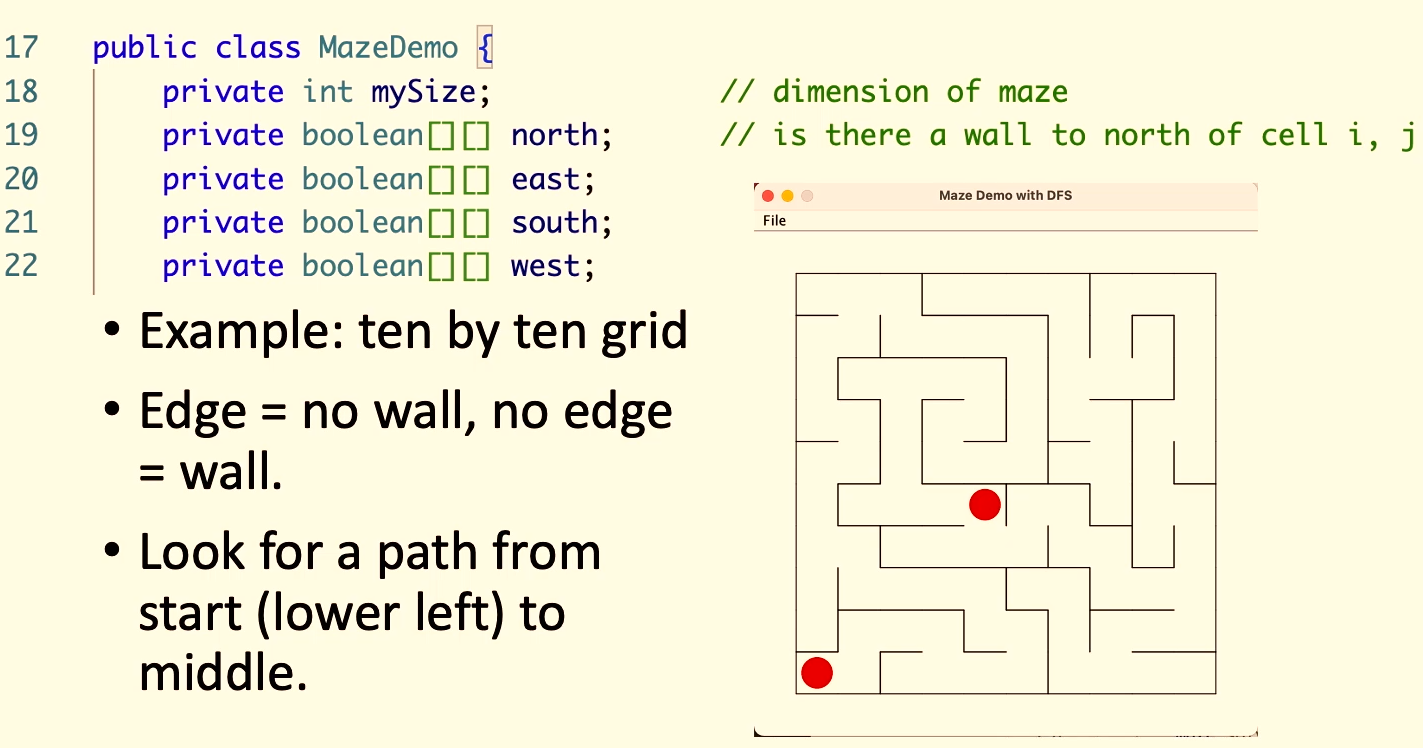
\includegraphics[scale=0.3]{img/grid_graph.png}
    \end{center}
    But remember that in a tree traversal, we recursively searched down and down until we hit a null node, in which case we backtrack up to look in another branch. For graphs, this is a bit more complicated, since we could go in loops. Therefore, we want to keep track of all the visited nodes to avoid infinite recursion. We have three base cases: 
    \begin{enumerate}
        \item If we search off the grid, then this is not a valid path 
        \item If we already explored here, then we don't want to repeat it 
        \item If we reached the goal of the maze, then we output the length of the path. 
    \end{enumerate}
    The recursive case would take each node and recurse on its 4 adjacent neighbors, if they are connected. So, the entire function, which takes in a location $(x, y)$ in the grid and the depth that it took to traverse to this point, would look like this: 
    \begin{lstlisting}

    private boolean[][] visited; 

    private int solveDFS(int x, int y, int depth) {
        if (x == 0 || y == 0 || x == mySize + 1 || y == mySize + 1) {
            return 0; 
        }
        if (visited[x][y]) return 0; 
        
        visited[x][y] = true; 
        
        if (x == mySize/2 && y == mySize/2) {
            return depth; 
        }
        
        if (!north[x][y]) { // if there is no wall above
            int d = solveDFS(x, y + 1, depth + 1); 
            if (d > 0) return d; 
        }
        if (!east[x][y]) {
            int d = solveDFS(x + 1, y, depth + 1); 
            if (d > 0) return d; 
        }
        if (!south[x][y]) {
            int d = solveDFS(x, y - 1, depth + 1); 
            if (d > 0) return d; 
        }
        if (!west[x][y]) {
            int d = solveDFS(x - 1, y, depth + 1); 
            if (d > 0) return d; 
        }
    }
    \end{lstlisting}
    Note that this algorithm recurses on each of the $N$ nodes $4$ times (for each direction, and each recursive call is $O(1)$), so the complexity is $O(N)$. 
  \end{example}

  Note that the main idea of DFS is to always explore a new adjacent vertex if possible, and if not, then backtrack to the most recent vertex adjacent to an unvisited vertex and continue. On the contrary, the main idea of BFS is to explore \textit{all} your neighbors before you visit any of your neighbors' neighbors. It exhaustively searches for the closest regions of your search space before you look any further. Unlike DFS, which finds the some arbitrary path to a node, BFS finds the shortest (perhaps nonunique) path to a node. This can be simply done with a queue. 

  \begin{definition}[BFS]
    The iterative version is shown.\footnote{The recursive version of BFS is very nontrivial.}
    \begin{lstlisting}
      visited = set() 
      def bfs(start): 
        toExplore = collections.deque() 
        current = start; 
        toExplore.append(current) 
        visited.add(current) 
        while toExplore: 
          current = toExplore.popleft() 
          # Do something 
          neighbors = ... 
          for neighbor in neighbors: 
            if neighbor not in visited: 
              visited.add(neighbor) 
              toExplore.append(neighbor)
    \end{lstlisting}
  \end{definition}

  \begin{theorem}[Runtime of BFS]
    The runtime of BFS is $O(n+m)$. 
  \end{theorem}
  \begin{proof}
    To get the running time, we know that each vertex is popped only once from the queue, giving us $O(n)$. For each pop, we are exploring all the neighbors of $V$. 
    \begin{align}
      O \bigg( \sum_{v \in V} | \text{neighbors of } v| + 1\bigg) & = O \bigg( \sum_{v \in V} d_v + 1 \bigg) \\
                                           & = O (2 |E| + |V|) = O(m + n )
    \end{align}
    which is linear in input size!  
  \end{proof}

  The more straightforward application is in reachability. 

  \begin{example}[Reachability]
    Given a directed graph and a node $v$, find all nodes that are reachable from $v$. 
  \end{example}

  \begin{exercise}
    Prove that in any connected undirected graph $G = (V, E)$ there is a vertex $v \in V$ s.t. $G$ remains connected after removing $v$. 
  \end{exercise}
  \begin{proof}
    Let $u$ be such a leaf node of $T$, and let $G'$ be the subgraph of $G$ resulting by removing $u$ and its incident edges from $G$.
    For sake of contradiction,\footnote{We provide an alternative direct proof as follows: Since $G$ is given to be connected, $T$ contains all vertices of $G$. Let $T'$ be the BFS tree minus $u$ and its single incident edge connecting it to its parent in $T$. Since $u$ is a leaf, $T'$ remains a connected tree with all other vertices of $G$. The edges of $T'$ exist in $G'$, so $G'$ is connected.} suppose $G'$ has more than one connected component.
    Let $C$ be a connected component in $G'$ that does not contain $s$, the root of the BFS tree $T$.
    Since $G$ was connected before the removal of $u$, it must be that every path from $s$ to any vertex $v$ in $C$ includes $u$ (otherwise there would remain a path from $s$ to $v$ in $G'$ and $s$ would be in $C$).
    Then $u$ is the only vertex not in $S$ with edges to vertices in $S$, so all vertices in $C$ must be ``visited'' during BFS only after visiting $u$. Furthermore, the vertices of $S$ must be in the subtree of $T$ rooted at $u$. But $u$ is a leaf, which is a contradiction.
  \end{proof}

  \begin{exercise}
    Two parts. 
    \begin{enumerate}
      \item Give an example of a strongly connected directed graph $G = (V, E)$ s.t. that every $v \in V$, removing $v$ from $G$ gives a directed graph that is not strongly connected. 
      \item In an undirected graph with exactly two connected components, it is always possible to make the graph connected by adding only one edge. Give an example of a directed graph with two strongly connected components such that no addition of one edge can make the graph strongly connected.
    \end{enumerate}
  \end{exercise}
  \begin{proof}
    Listed. 
    \begin{enumerate}
      \item A graph whose edges form a cycle, having at least three nodes.
      \item Two strongly connected components with no edges between them.
    \end{enumerate}
  \end{proof} 

  \begin{definition}[Search Trees]
    Once we have traversed a graph using BFS or DFS, we can label the directed path that this traversal algorithm takes into a \textbf{search tree}. If we look at the search trees generated by DFS and BFS, we can see that the path from A to C is always shorter for BFS than for DFS. 
    \begin{center}
      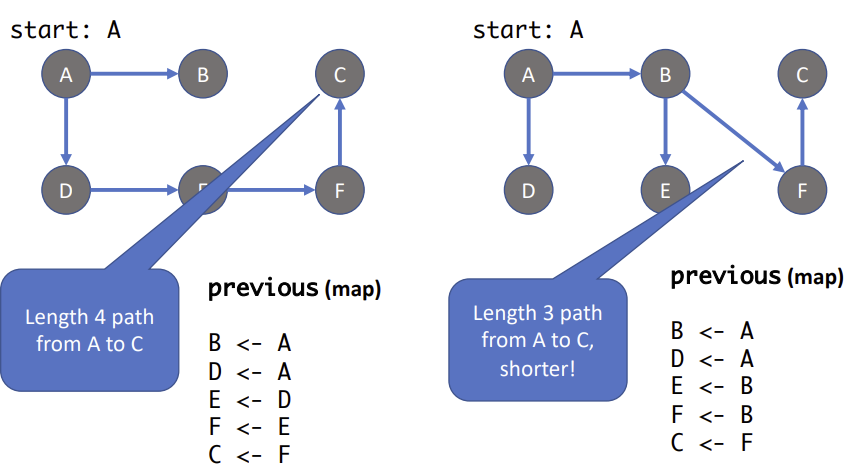
\includegraphics[scale=0.4]{img/search_trees.png}
    \end{center}
  \end{definition}

\subsection{Directed Acyclic Graphs and Topological Sorting}

  \begin{definition}[Directed Acyclic Graph]
    A DAG is a directed graph that has no cycles. Note that a DAG must have a node that has no in-edges. 
  \end{definition}

  To determine if a graph is a DAG, then we can brute force it by taking a node $s \in V$, running DFS/BFS, and if a neighbor is already in visited, return False. Then go through this for all starting nodes $s \in V$. This again has quadratic runtime. Can we do better? This introduces us to topological sorting. 

  It may be helpful to take a graph $G(V, E)$ and induce some partial order on the set of nodes $V$ based off of $E$. It turns out that we can do this for a specific type of graph. 
  
  \begin{definition}[Topological Sort]
    Given a directed acyclic graph (DAG), a linear ordering of vertices such that for every directed edge $u-v$, vertex $u$ comes before $v$ in the ordering is called a \textbf{topological sort}. It satisfies the facts: 
    \begin{enumerate}
      \item The first vertex must have an in-degree of $0$. 
      \item A topological sort is not unique. 
    \end{enumerate}

    \begin{figure}[H]
      \centering
      \begin{subfigure}[b]{0.48\textwidth}
      \centering
        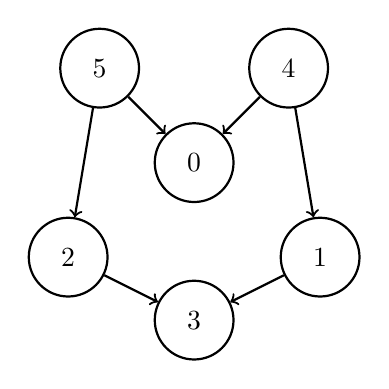
\begin{tikzpicture}[
            scale=0.8, 
            node/.style={circle, draw, thick, minimum size=1.0cm}, 
            edge/.style={->, black, thick}
        ]

        % Center node
        \node[node] (n0) at (0,0) {0};

        % Upper nodes
        \node[node] (n5) at (-1.5,1.5) {5};
        \node[node] (n4) at (1.5,1.5) {4};

        % Lower nodes
        \node[node] (n2) at (-2,-1.5) {2};
        \node[node] (n1) at (2,-1.5) {1};
        \node[node] (n3) at (0,-2.5) {3};

        % Directed edges
        \draw[edge] (n5) -- (n0);
        \draw[edge] (n4) -- (n0);
        \draw[edge] (n5) -- (n2);
        \draw[edge] (n4) -- (n1);
        \draw[edge] (n2) -- (n3);
        \draw[edge] (n1) -- (n3);
        \end{tikzpicture}
        \caption{This graph can have the two (not exhaustive) topological sortings $[5, 4, 2, 3, 1, 0]$ and $[4, 5, 2, 3, 1, 0]$.}
        \label{fig:top_sort_not_unique}
      \end{subfigure}
      \hfill 
      \begin{subfigure}[b]{0.48\textwidth}
      \centering
        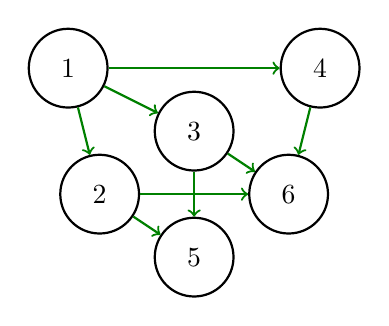
\begin{tikzpicture}[
            scale=0.8,
            node/.style={circle, draw, thick, minimum size=1.0cm},
            edge/.style={->, green!50!black, thick}
        ]

        % Center and bottom nodes
        \node[node] (n3) at (0,0) {3};
        \node[node] (n5) at (0,-2) {5};

        % Left side nodes
        \node[node] (n1) at (-2,1) {1};
        \node[node] (n2) at (-1.5,-1) {2};

        % Right side nodes
        \node[node] (n4) at (2,1) {4};
        \node[node] (n6) at (1.5,-1) {6};

        % Directed edges ensuring unique topological order
        \draw[edge] (n1) -- (n2);
        \draw[edge] (n1) -- (n3);
        \draw[edge] (n1) -- (n4);
        \draw[edge] (n2) -- (n5);
        \draw[edge] (n3) -- (n5);
        \draw[edge] (n3) -- (n6);
        \draw[edge] (n4) -- (n6);
        \draw[edge] (n2) -- (n6);

        \end{tikzpicture}
        \caption{This graph can have the two (not exhaustive) topological sortings $[1, 4, 2, 3, 6, 5]$ and $[1, 4, 3, 2, 6, 5]$.}
        \label{fig:top_sort_unique}
      \end{subfigure}
      \caption{Examples of topological sortings of different graphs. }
      \label{fig:top_sort}
    \end{figure}
  \end{definition}

  To determine if a graph is a DAG, note the following theorem. 

  \begin{theorem}[Topological Order and DAGs]
    $G$ has a topological order if and only if it is a DAG. 
  \end{theorem}
  \begin{proof}
    To prove that a DAG has a topological order, we use induction. Pick a $v$ such that its indegree is $0$. Then, delete $v$, and therefore $G \setminus v$ is also a DAG with a topological order since we are only deleting edges. We keep going. 
  \end{proof}

  Therefore, if we can successfully topologically sort, we know it is a DAG. So we can kill two birds with one stone. Let's see how this is implemented. We can do it iteratively and recursively (the proof above should hint that this can be recursive). 

  \begin{algo}[Iterative Topological Sort, Determine If Graph is DAG]
    The general idea is that we first find the node that as $0$ in-degree. From here, we can do DFS, and when we run out of neighbors to explore, then we push this into a queue. This is essentially a post-order traversal, where at the end are going to be the end nodes with no more neighbors, and the node we started from will be added last. Then we loop through and do this for all start nodes. We first need a slightly modified form of DFS. 

    \begin{algorithm}[H]
      \label{alg:iterative_top_sort}
      \begin{algorithmic}[1]
        \Require{Nodes $V$, adjacency list $E$}
        \State visited $\gets$ set()
        \State res $\gets$ stack() 
        \State is\_acyclic $\gets$ True

        \Function{DFS}{$v \in V$}
          \If{$v \neq $ visited}
            \State add $v$ to visited 
            \State $N_v \gets$ neighbors of $v$ 
            \For{$n \in N_v$}
              \If{$n \in $ visited} 
                \State is\_acyclic $\gets$ False 
              \EndIf
              \State \Call{DFS}{$n$}
            \EndFor 
            \State push $v$ onto res
          \EndIf
        \EndFunction

        \State 

        \Function{TopologicalSort}{V, E}
          \For{$v \in V$} 
            \State DFS($v$)
          \EndFor
          \If{! is\_acyclic}
            \State \Return{False}
          \EndIf
          \State \Return{reversed of res}
        \EndFunction
      \end{algorithmic}
    \end{algorithm}
    Note that this runtime is $O(|V| + |E|)$ since we are just running DFS with a constant amount of work on top of each call. 
  \end{algo}

  \begin{algo}[Recursive Topological Sort]
    We want to see that while $G$ is nonempty, we want to find the $v \in V$ such that it has indegree $0$. Then place $v$ next in order, and then delete $v$ and all edges out of $v$. The problem is finding which vertex has indegree $0$ (if we brute force it by looking through all remaining nodes and edges, you have quadratic runtime). To do this fast, the idea is 
    \begin{enumerate}
      \item initially scan over all edges to store the indegrees of every node to a list \texttt{indeg}. 
      \item store all nodes with indegree $0$ to a queue. 
      \item Run through the queue, and during each loop, when we remove a node, we look at all of its out-nodes $s$ and decrement \texttt{indeg[s]}. If \texttt{indeg[s] = 0}, then add it to the queue. 
    \end{enumerate}
    \begin{algorithm}[H]
      \label{alg:recursive_top_sort}
      \begin{algorithmic}[1]
        \Require{Nodes $V$, Edges $E$}
        \State $q \gets$ queue() 
        \State indeg $\gets$ list() 
        \State visited $\gets$ 0
        \Function{Recur}{x}
          \State initialize the indeg and $q$ 

          \While{q is nonempty} 
            \State $v \gets$ pop(q) 
            \State visited += 1 
            \For{each $w \in E[v]$} 
              \State indeg[w] -= 1 
              \If{indeg[w] = 0} 
                \State push w into q 
              \EndIf
            \EndFor
          \EndWhile

          \If{visited != |V|} 
            \State \Return{False}
          \EndIf

          \State \Return{True}
        \EndFunction
      \end{algorithmic}
    \end{algorithm}
    Notice that the inner for loop is $O(d(v) + 1)$, while we run over all $n$. So really, we are doing $O(n(d(v) + 1)) = O(m + n)$, where the plus $n$ comes from the constant work we are doing for each node. Note that if we have a non-DAG, then at some point the queue will be empty but we haven't processed all the vertices, at which point we can declare failure. 
  \end{algo}

  To end this, we can make a general statement about all directed graphs. 

  \begin{theorem}
    Every directed graph is a DAG of strongly connected components (SCC). 
  \end{theorem}

  This gives us a way to represent a directed graph with a collection of DAGs.\footnote{In fact, this Kosaraju's algorithm, can be done in linear time, though it is highly nontrivial.} An extension of topological sort is making a \textit{BFS tree}, which partitions a graph into layers that represent the number of steps required to go from a source vertex to a node. 

  \begin{algo}[BFS Tree]
    To construct a BFS tree, we just need to slightly modify the original BFS code.
    \begin{algorithm}[H]
      \label{alg:bfs_tree}
      \begin{algorithmic}[1]
        \Require{Nodes $V$, adjacency list $E$}
        \State visited = set() 
        \State layers = $\{v : 0 \mid v \in V \}$
        \Function{BFS}{start}
          \State layer $\gets 0$ 
          \State toExplore $\gets$ queue() 
          \State add (start, layer) to toExplore 
          \State add start to visited
          \While{toExplore} 
            \State curr, layer = pop from toExplore 
            \State layers[curr] = layer 
            \For{$n \in$ neighbors of curr} 
              \If{$n \not\in$ visited} 
                \State add $n$ to visited 
                \State add $(n, layer+1)$ to visited 
              \EndIf
            \EndFor
          \EndWhile 
        \EndFunction
      \end{algorithmic}
    \end{algorithm}
    This is simply BFS with constant extra work so it is $O(n + m)$. 
  \end{algo}

  So, a BFS tree is really just another way to topologically sort. Note the following properties. 
  \begin{enumerate}
    \item In a directed graph, no nodes can jump from layer $i$ to layers $j > i+1$, since if it could, then it would be in layer $i+1$. However, nodes can jump from layer $j$ back to any layer $i < j$, even skipping layers. 
    \item In a directed graph, going forward is the same as going back, so nodes can jump at most one layer forwards or backwards. 
  \end{enumerate}


  \begin{exercise}[DPV 3.16]
    Suppose a CS curriculum consists of $n$ courses, all of them mandatory. The prerequisite graph $G = (V,E)$ has a node for each course, and an edge from course $v$ to course $w$ if and only if $v$ is a prerequisite for $w$. Note this is a directed acyclic graph (DAG). In order for a student to take a course $w$ with prerequisite $v$, they must take $v$ in an earlier semester. Find an algorithm that works directly with this graph representation, and computes the minimum number of semesters necessary to complete the curriculum, under the assumption any number of courses can be taken in one semester. The running time of your algorithm should be $O(n+m)$, where $n$ and $m$ are the numbers of vertices and edges in $G$, respectively.
  \end{exercise}
  \begin{proof}
    For each vertex, we want to find the longest path leading to it: if there is a path leading to a node, then all of the courses in the path should be taken sequentially. Perform a topological sort of $G$'s nodes and label them $1$ through $n$. Then, we go through the nodes in the resulting topological order. For each vertex, we assign the minimum number of semesters required to take it: if there are no prerequisites, we assign 1, and if there are prerequisites, we assign 1 plus the maximum value assigned to its prerequisite nodes.
    
    \textit{Implementation details}: If the input is in adjacency list format, then we do not have access to the \emph{incoming} edges to a node (its prerequisites). By exploring the entire graph with BFS calls, we can compute the list of incoming edges to every vertex in $O(n+m)$ time. These details are not required. If the input is in adjacency matrix format, for each node it takes $O(n)$ time to find its incoming edges, so the total running time is $O(n^2)$.
  \end{proof}

  \begin{exercise}[DPV 3.22] 
    Give an efficient algorithm that takes as input a directed graph $G = (V,E)$, and determines whether or not there is a vertex $s \in V$ from which all other vertices are reachable.
  \end{exercise}
  \begin{proof}
    We first build the DAG representation of the SCCs of $G$ in $O(m+n)$ time, as described in lecture. This graph is a DAG where each SCC of $G$ is represented by a single node. We return true if this DAG has exactly one node with no incoming edges (i.e., exactly one source node), and return false otherwise.

    \textit{Correctness.} Let $u$ be a vertex in an SCC that is a source node in the DAG representation. If there is a path in $G$ from a vertex $v$ not in the SCC of $u$ to $u$, then there must be an edge (corresponding to an edge in this path) into the SCC of $u$ in the DAG, which contradicts that the node has no incoming edges. Thus, if there are two source SCCs in the DAG, no vertex of $G$ can reach all vertices; in particular, no vertex can reach the vertices in both of the source SCCs. Thus we correctly return false if there are multiple source SCCs. 
    
    On the other hand, if there is a single source SCC in the DAG, we claim that every vertex in the SCC can reach every other vertex in $G$, in which case our algorithm correctly returns true. Every other SCC in the DAG is not a source, so it has an incoming edge.\footnote{The following argument can be made formal with induction.} Consider starting at an SCC in the DAG, picking an incoming edge to the SCC, and then repeating this process from the SCC from which the edge was leaving. This process stops when we reach an SCC without incoming edges. In this case there is exactly one source SCC, so this process will arrive at the single source SCC when starting from any SCC in the DAG. This implies there is a path from the unique source SCC to every other SCC in the DAG, and thus every vertex of the source SCC can reach all vertices in all SCCs of $G$; that is, all vertices of $G$.
  \end{proof}

  \begin{exercise}[DPV 3.19]
    You are given a binary tree $T = (V, E)$ with designated root node with $n = |V|$ vertices which are the integers from $1$ to $n$. In addition, there is an array $x[1..n]$ of values where $x[u]$ is the value of vertex $u \in V$. Define a new array $z[1..n]$ where, for each $u \in V$,	
    \begin{equation}
      z[u] = \max \{ x[v] \mid \text{$v$ is a descendant of $u$}\}
    \end{equation}
    That is, $z[u]$ is the maximum $x$-value of all vertices in the subtree of $T$ rooted at $u$. Note that, by definition, any node is a descendant of itself. Describe an $O(n)$-time algorithm which calculates the entire $z$-array.
  \end{exercise}
  \begin{proof}
    We propose the following recursive algorithm performs a \emph{postorder} traversal of the tree and populates the values of the $z$-array in the process:
    \begin{lstlisting}
      computeZ(u):
        maxVal = x[u]
        if u.left is not null:
          computeZ(u.left) # compute z for all descendants of u.left
          maxVal = max(z[u.left], maxVal)
        if u.right is not null:
          computeZ(u.right) # computes z for all descendants of u.right
          maxVal = max(z[u.right], maxVal)
        z[u] = maxVal
    \end{lstlisting}
    We initially call \texttt{computeZ} on the root node of $T$.        The algorithm takes $O(1)$ time per node, which is $O(n)$ overall\footnote{This algorithm can also be described as a modified version of the so-called \emph{depth-first search} (DFS) graph traversal algorithm, which is different from BFS.}
  \end{proof}

  \begin{exercise}
    Your data center needs to run a number of jobs (compute requests) numbered $1, 2, \dots, n$. These are specified in a list of $m$ tuples where $(i, k)$ means that job $i$ must be completed before job $k$ can run. A given job may have multiple dependencies; for example, you might have constraints $(1, 4), (2, 4), (3, 4)$ that all of jobs $1, 2, \mbox{ and } 3$ must be completed before $4$ can run.
    \begin{enumerate}
      \item Describe an $O(n+m)$ runtime algorithm that determines whether it is possible to execute all of the jobs, and if so, determines a valid order in which to execute the jobs one at a time. \textit{Hint. How to relate SCCs to cycles?}
      \item Suppose you have $n$ identical servers (so that if there were no constraints you could simply run each job on a separate server). Suppose every job has the same runtime $R$. Describe an $O(n+m)$ runtime algorithm to compute the total runtime that will be necessary to run all of the jobs in a valid order.
    \end{enumerate}
  \end{exercise}
  \begin{proof}
    For this question we define a graph $G = (V, E)$ where there is a vertex for every job $1, \dots, n$ and an edge from $i$ to $k$ for every listed dependency (where $k$ depends on $i$).

    \begin{enumerate}
        \item We note that a sequence of jobs can be executed if and only if there is no circular dependency. In the language of graphs, this requires that $G$ be free of cycles. To this end, it suffices to propose an algorithm that runs in $\mathcal{O}(m+n)$. We will use Kosaraju's SCC algorithm. We prove the following claim:

        \centerline{Any SCC with $\geqslant 2$ vertices contain a cycle.}
                    \vspace{5pt} 
  
        To see this, consider any distinct $u,v$ in this SCC. Let $p_{u,v}$ and $p_{v,u}$ be the paths from $u$ to $v$ and backwards, respectively. Now concatenate the paths and get a walk that starts from $u$ and ends at $u$. Note that each vertex appears at most once in $p_{u,v}$ and in $p_{v,u}$, so in the combined walk, it appears at most twice. Consider the set of vertices that are revisited in this walk --- clearly, $u$ is one of them and is the latest one to be revisited. There must exist a vertex $w$ that was the \textit{first} to be revisited. Then, the section of the walk between the two visits of $w$ form a cycle by definition: it starts from $w$, ends at $w$, and does not repeat any other vertices. This proves the claim. And to go back to our problem, the following are equivalent: 
        \begin{enumerate}
          \item jobs can be executed 
          \item no cycles in $G$ 
          \item each SCC obtained from Kosaraju is a singleton
        \end{enumerate}

        \item We first run the algorithm from part (a) to check if it is possible and to find a valid order of the jobs if so. Then define an array $L$ of length $n$. We will compute $L[k]$ as the length of the longest dependency chain prior to $k$. Loop over the $k$ jobs in topological order. For each, compute $L[k] = 0$ if $k$ has no dependencies, or $L[k] = 1 + \max_{(i, k)} L[i]$ otherwise. Finally, return $\max_{k} L[k]$. 
    \end{enumerate}
    
  \end{proof}

\subsection{Bipartite Graphs}

  Now we shall see a further application of BFS trees. 

  \begin{definition}[Bipartite Graph]
    A \textbf{bipartite graph} is an undirected graph $G(V, L)$ where we can partition $V = L \sqcup R$ such that for all $e = \{u, v\} \in E$, we have $u \in L, v \in R$.  
  \end{definition}

  We would like to devise some method to determine if an arbitrary graph is bipartite. 

  \begin{theorem}
    $G$ is bipartite if and only if all cycles in $G$ are even length. 
  \end{theorem}
  \begin{proof}
    Proving $(\implies)$ is quite easy since if we suppose $G$ has an odd length cycle, then we start packing vertices of a cycle into $L, R$, but by the time we came back to the start, we are forced to pack it into the wrong partition! 

    The converse is quite hard to prove, and we'll take it at face value. 
  \end{proof}

  Now in practice, how would we determine if all cycles are even length? This is where BFS shines. 

  \begin{algo}[Determine Bipartite On All Cycles of Even Length]
    The general idea is we first run BFS on the graph starting at $s \in V$, which divides it up into layers $L_1, \ldots, L_l$ representing the shortest path from $s$. Then for each layer $L_i \subset V$, we check if there are connections between two vertices $x, y \in L_i$. If there are connections, then this is not bipartite. If there are none, then this is bipartite since we can then color it. 

    \begin{algorithm}[H]
      \label{alg:determine_bipartite}
      \begin{algorithmic}[1]
        \Require{Nodes $V$, adjacency list $E$}
        \State visited = set() 
        \State layers = $\{v : 0 \mid v \in V \}$
        \Function{BFS}{start}
          \State layer $\gets 0$ 
          \State toExplore $\gets$ queue() 
          \State add (start, layer) to toExplore 
          \State add start to visited
          \While{toExplore} 
            \State curr, layer = pop from toExplore 
            \State layers[curr] = layer 
            \For{$n \in$ neighbors of curr} 
              \If{$n \not\in$ visited} 
                \State add $n$ to visited 
                \State add $(n, layer+1)$ to visited 
              \EndIf
            \EndFor
          \EndWhile 
        \EndFunction

        \State 

        \Function{Bipartite}{V, E}
          \State BFS(v) for some $v \in V$ 
          \For{$(u, v) \in E$} 
            \If{layers[u] == layers[v]} 
              \State \Return{False} 
            \EndIf 
          \EndFor 
          \State \Return{True}
        \EndFunction
      \end{algorithmic}
    \end{algorithm}
    Therefore, we run BFS, which is $O(n+m)$, and then to compare the edges, it is $O(m)$. 
  \end{algo}

  Bipartiteness is actually a special case of \textit{coloring problems}. Given a graph with $k$ colors, can I color it so that every neighbor has a different color than the original node? It may seem like at first glance that we can do the same method and look at the layers again, but it turns out that 3-coloring is hard. More specifically it is an NP-complete problem, which colloquially means that there isn't much of a better way than a brute-force solution. However, it turns out that according to the \textit{4 color theorem}, any map can be colored with 4 colors. 

\subsection{Strongly Connected Graphs}

  Now how do we find out if a directed graph is strongly connected? The straightforward solution would be to take each vertex $v \in V$, run BFS to find the set of vertices reachable from $v$, and do this for every vertex. The total running time is $O(n(n+m))$, which is quadratic. Note that for an undirected graph this is trivial since we just run DFS/BFS once. 

  \begin{theorem}
    $G$ is strongly connected if and only if for any $v \in V$, 
    \begin{enumerate}
      \item all of $V$ is reachable from $v$. 
      \item $v$ is reachable from any $s \in V$
    \end{enumerate}
  \end{theorem}

  \begin{algo}[Determine if Graph is Strongly Connected]
    Using the theorem above, we can run BFS/DFS twice: one on the original graph and one on the reversed graph, consisting of all edges directed in the opposite direction. 
    \begin{algorithm}[H]
      \label{alg:strongly_connected}
      \begin{algorithmic}[1]
        \Require{Nodes $V$, Adjacency list $E$}
        \Function{StronglyConnected}{$s \in V$}
          \State visited $\gets$ set() 
          \State BFS(s) 
          \If{visited != $V$} 
            \State \Return{False}
          \EndIf
          \State visited $\gets$ set() 
          \State reverse all edges in $E$ 
          \State BFS(s) 
          \If{visited != $V$} 
            \State \Return{False}
          \EndIf
          \State \Return{True}
        \EndFunction
      \end{algorithmic}
    \end{algorithm}
    The running time is just running BFS twice plus the time to reverse the edges, so it is $O(n+m)$. 
  \end{algo}

\subsection{Shortest Path}

  In the shortest path, you are given a \textit{weighted} (positive integer) directed graph and your goal is to find a path from $s$ to $t$ with the smallest length. This is where we use Dijkstra's. What we can do to brute force is just replace a edge with length $k$ to $k$ edges of length $1$, and we run BFS on this. However, this is not efficient since the weights can be unbounded. This is where we introduce Dijkstra. The following is how it is introduced in class. 

  \begin{algo}[General Dijkstra]
    We can keep a temporarily list $\pi$ of the shortest path we have found so far, and a permanent list \texttt{dist} keeping track of all paths we know are for sure the shortest path. 
    \begin{algorithm}[H]
      \label{alg:dik_in_class}
      \begin{algorithmic}[1]
        \Require{Graph $G(E, V)$}
        \State $S \gets \{s\}$  \Comment{set of nodes that we know for sure is shortest}
        \State dist[s] = 0 and the rest very large numbers \Comment{our final list}
        \State $\pi[v] = w_{sv}$ for all $v \in V$ \Comment{initialize list with neighboring nodes from start $s$}
        \Function{Dijkstra}{s}
          \State $u = \mathrm{argmin}_{v \notin S} \pi[v]$ \Comment{Find node having minimum accum weight so far}
          \State add $u$ to $S$ \Comment{This node must be shortest so add to $S$}
          \State $\mathrm{dist}[u] = \pi[u]$ \Comment{Now we can update its shortest path in dist}
          
          \For{$v \not\in S$} \Comment{Look at all neighbors of $u$ and update those not in}
            \State $\pi[v] \gets \min\{\pi[v], d[u] + w_{wv}\}$ \Comment{$S$ since those in $S$ are all guaranteed to be shortest}
          \EndFor
        \EndFunction
      \end{algorithmic}
    \end{algorithm}
  \end{algo}

  The problem is line 5 above. We don't want this linear search time since it makes the whole thing quadratic, so rather than a list, we can implement a heap, resulting in the code below. 

  \begin{algo}[Dijkstra's Algorithm]
    The general idea is to run a graph traversal like BFS but when you reach a new vertex $v$, you can store the accumulated time it took to get to $v$ and store for all neighbors the accumulated time it will take to get to each of those neighbors. If it is less than what we have currently, then we have found a shorter path and we should update this. 
    \begin{algorithm}[H]
      \label{alg:dijkstra}
      \begin{algorithmic}[1]
        \Require{Nodes $V$, Edges $E$}
        \Function{Dijkstra}{s}
          \State dist $\gets$ list of size $|V|$ with $+\infty$ \Comment{Initialize list of big nums representing shortest distances}
          \State dist[$s$] $\gets$ 0 \Comment{The starting node has dist $0$}
          \State predecessors $\gets$ $\{v : None \mid v \in V \}$ \Comment{predecessors of each node for path tracking}
          \State toExplore $\gets$ minheap() \Comment{A priority queue of (weight, node)}
          \State add $(0, s)$ to toExplore \Comment{You want to explore this first}

          \While{toExplore} 
          \State (curr\_dist, curr\_node) $\gets$ pop from toExplore  \Comment{pop from toExplore}
            \If{curr\_dist > dist[curr\_node]}  \Comment{If this distance is greater than what}
              \State continue \Comment{I already have then not worth exploring}
            \EndIf 

            \For{neighbor, weight $\in$ E[curr\_node]} \Comment{Look at each neighbor}
              \State new\_dist $\gets$ curr\_dist + weight \Comment{The distance to getting to neighbor from now}
              \If{new\_dist < dist[neighbor]} \Comment{If this new dist is shorter than what we have}
                \State dist[neighbor] = new\_dist \Comment{Update best distance}
                \State predecessors[neighbor] = curr\_node \Comment{Update its predecessor}
                \State push (new\_dist, neighbor) onto toExplore \Comment{Should prob explore from here}
              \EndIf
            \EndFor
          \EndWhile
          \State \Return{distances, predecessors}
        \EndFunction
      \end{algorithmic}
    \end{algorithm}

    You essentially push $n$ times and pop $m$ times, and the time per push and pop is $\log_2 (n)$. Therefore, the total time to push is $n \log(n)$ and to pop is $m \log (n)$, making the total runtime $O(log(n) (n+m))$. 
  \end{algo}

  The first example gotten in class ignores the distances and just attempts to modify the distances in the heap itself (through the decrease key operation). This takes $2 \log_2 (n)$, but if we use a heap with $d$ children, we can modify the runtime to $d \log_d (n)$. Therefore, the total runtime with tunable parameter $d$ is 
  \begin{equation}
    O\big( (m + nd) \log_d (n)\big)
  \end{equation}
  which can be minimized if we set $d = m/n$, so $O(m \log_{m/n} n)$, where for dense graphs $m/n$ is large and so it can behave roughly in linear time $\Theta(m)$. 

  \begin{exercise}
    Let $G = (V,E)$ be a weighted strongly connected directed graph with positive edge weights. Let $v_0$ be a specific vertex. Describe an algorithm that computes the \textbf{\textit{cost}} of the shortest walk between every pair of vertices of $G$, with the restriction that each of these walks must pass through $v_0$ (that is, for every distinct pair $u, v \in V$, among all walks from $u$ to $v$ that pass through $v_0$, compute the cost of the shortest walk). Describe the algorithm, analyze its runtime complexity, and briefly explain (not a formal proof) why it is correct. Try to give an algorithm that runs in $O (|E|\log(|V|) + |V|^2)$ time. As usual, you may use any algorithm as described in lecture without restating it or arguing for its correctness.
  \end{exercise}
  \begin{proof}
    The high level idea is to decompose any qualifying $u\to v$ walk into the combination of two paths $u\to v_0\to v$, where we try to minimize the cost of both subpaths. It's easy to compute the minimum cost of $v_0\to v$ for all $v$: running Dijkstra once over the graph suffices. The first half, $u\to v_0$, is the nuisance since we need to calculate this quantity for every $u\in V$. Solution? Observe that the destination node $v_0$ is fixed! We flip the direction, define a ``reverse graph'' $G^{-1}$ where each edge carries its original weight but points in the other direction. Then, any cheapest $v_0\to u$ path in $G^{-1}$ would correspond to the cheapest $u\to v_0$ path in $G$, with matching total costs.  
  \end{proof}

  \begin{exercise}
    Let  $G=(V, E)$ be a directed, weighted graph with $|V|= n$ and $|E|=O(n)$ (that is, the graph is sparse). Let $s$ be a vertex in $V$. How quickly can the cost of the following shortest paths be computed under the given conditions? Just note the runtime and be prepared to explain. All of these can be solved using a single call to a shortest-path algorithm if provided the correct input graph (not necessarily the given one).
    \begin{enumerate}
      \item Compute the shortest path distance from some $s$ to all other vertices in $G$ under the condition that the weight of every edge is a positive integer $\le  10$.
      \item Compute the shortest path distance \textit{to} a target $t$ from all possible source vertices $s$ in a graph with positive edge weights.
    \end{enumerate}
  \end{exercise}
  \begin{proof}
    Listed. 
    \begin{enumerate}
      \item Since all weights are integer and uniformly bounded, we convert $G$ into an unweighted graph and apply BFS. Construct unweighted $G'=(V', E')$ as follows: for each directed edge $(u\to v \in E$, put a series of dummy nodes between $u,v$ in $G'$ so that the distance from $u$ to $v$ in $G'$ is precisely the integer weight $w(u,v)$ of $u\to v$ in $E$. Now $G$ has at most $10n$ nodes and $10n$ edges. So BFS runs in $O(\lvert V'\rvert  + \lvert E'\rvert ) = O(n)$.
      \item Construct the reversed graph $G^{-1}$ and run $\mathrm{Dijkstra}(G^{-1}, t)$. This finishes in $\mathcal{O}((m+n) \log n) = O(n\log n)$ time since $G$ is sparse.
    \end{enumerate}
  \end{proof}

  \begin{exercise}
    Let $G=(V,E)$ be an undirected, weighted graph with non-negative edge weights. Let vertices $s,t\in V$ be given. Describe an algorithm that efficiently solves the following questions.
    \begin{enumerate}
      \item Find the shortest/cheapest $s-t$ walk with an even number of edges.
      \item Find the shortest/cheapest $u-v$ walk with a number of edges of form $6k+1, k\in \mathbb{N}$. 
    \end{enumerate}
  \end{exercise}
  \begin{proof}
    Listed. 
    \begin{enumerate}
      \item The key observation is that as we travel on $G$, the number of edges we have travelled along alternates between being odd and even. Furthermore, the very same vertex may correspond to both even and odd: for example if we walked along $u\to v\to w\to u$, then initially we travelled for $0$ edges, but upon return we travelled a total of $3$ edges. We need a way to distinguish them. The solution? Duplicate each vertex into two categories: ``odd'' and ``even.''

      We construct a new graph $G' = (V', E')$ by duplicating every vertex $v\in V$, labeling one of them as $v_{\text{odd}}$ and the other $v_{\text{even}}$. For each edge $(u,v)\in E$, add two edges $(u_{\text{odd}}, v_\text{even})$ and $(u_{\text{even}}, v_{\text{odd}})$ to $E'$, both with the same as $(u,v)\in E$. 

      Clearly, $\lvert V'\rvert  = 2 \lvert V\rvert $ and $\lvert E'\rvert  = 2 \lvert E\rvert $. What would edges look like in $G'$? By construction, the two endpoints of an edge in $G'$ have different subscripts, one with ``odd,'' the other ``even.'' This agrees with our previous observation on the original $G$ that as we walk along the graph, the distance we have so far travelled alternates between even and odd. It follows that, starting from $s_\text{even}$, a vertex $v_\text{even}\in V'$ (resp. $v_\text{odd}$) is only reachable via even (resp. odd) number of edges. 

      On the other hand, also notice that there is a natural correspondence between edges in $G'$ and $G$: $(u_\text{odd}, v_\text{even})\in E'$ corresponds to $(u,v)\in E$. This means a \textit{path} in $G'$ naturally corresponds to a walk in $G$, e.g.:

      \[u_\text{even} \to v_\text{odd} \to w_\text{even} \to u_{\text{odd}} \to t_\text{even} \qquad \text{corresponds to}\qquad u\to v\to w \to u\to t.\]

      Combining both observations above, there exists an $s-t$ walk in $G$ with an even number of edges if and only if there is a path in $G'$ from $s_\text{even}$ to $t_\text{even}$. The rest is simple: run a pathfinding algorithm on $G'$. The weights are non-negative, so we use Dijkstra's algorithm. 

      Total runtime? Time to construct $G'$ involves $\lvert V'\rvert = 2\lvert V\lvert$ vertices and $\lvert E'\rvert = 2\lvert E\rvert$ edges. This is dominated by running Dijkstra on $G'$, which takes $O((|V'| +\lvert E'\rvert )\log \lvert V'\rvert) = O((|V|+\lvert E\rvert)\log \lvert V\rvert)$ time. Finally, transforming the path in $G'$ back to a walk in $G$ takes linear time w.r.t. the path length (one step for each edge), which is bounded by $O(\lvert E'\rvert)$.  So overall most work is dominated by Dijkstra's algorithm and the overall algorithm runs in $O((|V|+\lvert E\rvert) \log \lvert V\rvert)$.

      \item Same idea but make 6 copies of the graph. 
    \end{enumerate}
  \end{proof}

  \begin{exercise}
    Suppose that in addition to having edge costs $\{l_e:e\in E\}$, a graph also has vertex costs $\{c_v:v\in V\}$. Now define the cost of a path to be the sum of its edge lengths, \textit{plus} the costs of all vertices on the path. Give an efficient algorithm for finding the minimum cost path from $s$ to $t$. You may assume edge costs and vertex costs are all nonnegative.
  \end{exercise}
  \begin{proof}
    Using the generic approach, we can use $\text{cost}_u(v)=\text{cost}(u)+w(u,v)+c_v$ to solve this problem. Alternatively, for each edge $(u,v)$ we can update its weight to $w(u,v)+c_v$ and run Dijkstra on this updated graph, which gives an equivalent mathematical formulation.
  \end{proof}

\subsection{Negative Weighted Graphs} 

  Now let's extend this problem to find the shortest path in negative weighted graphs. Before we think of a solution, we must make sure that there is no cycle that has a negative accumulated path. Otherwise, this problem becomes ill-defined, so we first assume that such a shortest path exists. 

  At first glance, we may just think of adding $\min(v)$, the minimum value to every node so that this now just becomes a regular positive graph and run BFS on it. However, this does not work since we are not adding a constant number over all paths (it is proportional to the number of nodes in the path). 

  Another way we can think of is just run Dijkstra. However, if it is looking at two paths. We can have $s \xrightarrow{2} b$ and $s \xrightarrow{5} a \xrightarrow{-4} b$. Dijkstra will immediately go to $b$ thinking that it is the shortest path, since that's how far it see. So we need to look far into the future. Therefore, after an arbitrarily long path length, you could get a negative length that just kills your accumulator.  

  We use the Bellman equations, which could be solved using dynamic programming like we've seen before. 

  \begin{theorem}[Bellman Equations]
    We write the \textbf{Bellman equations}. 
    \begin{align}
      d[v] & = \min_{w} \{ d[w] + l_{w v}\}
    \end{align}
    with $d[s] = 0$ for the starting vertex. The solution has a unique solution that finds the shortest path from $s$ to any $v \in V$.    
  \end{theorem}
  \begin{proof}
    Note that $d[w] + l_{wv}$ is the length from some path from $s \mapsto v$ that goes through $w$. The minimum of it must be the shortest path over all $w \in V$. Suppose the shortest path goes through fixed $x$. If there exists a shorter path from $s \mapsto x$, then replace $d[x]$ by this shortest path. Therefore, 
    \begin{equation}
      d[v] = d[x] + l_{xv} \leq d[w] + l_{wv} \implies d[v] = \min_{w} \{d[w] + l_{w v}\}
    \end{equation}
    To prove uniqueness, suppose there are some other solutions $\pi$ where $\pi[v] \neq d[v]$ for some $v$. But this cannot be the case by definition since $d[v] <= \pi[v]$ for all $v$. 
  \end{proof}

  \begin{theorem}
    Given the shortest paths, we can lay out this graph like a tree where $l_{ab} = l_{a a_1} + l_{a_1 a_2} + \ldots + l_{a_l b}$. 
  \end{theorem}

  So how do we actually implement this? 

  \begin{algo}[Shortest Path in Possibly Negative Weighted Graph]
    \begin{algorithm}[H]
      \label{alg:neg_weighted_short_path}
      \begin{algorithmic}[1]
        \Require{Nodes $V$, Edges $E$}
        \Function{ShortPath}{V, E}
          \State res $\gets$ list(0) of large numbers of size $|V|$. 
          \State res[$s$] = 0
          \State predecessors $\gets \{v : None | v \in V\}$

          \While{$\exists (u, v)$ s.t. res[v] > res[u] + $l_{u v}$ } 
            \State res[$v$] $\gets$ res[u] + $l_{uv}$
            \State predecessor[v] $\gets$ u
          \EndWhile

        \EndFunction
      \end{algorithmic}
    \end{algorithm}
    This is guaranteed to converge and stop after a finite number of steps since at every iteration, a path will either 
    \begin{enumerate}
      \item get updated from infinity to a path length 
      \item get reduced from a path length to a shorter path length
    \end{enumerate} 
    And we will have to reach the shortest path length at which point we can't reduce it further.\footnote{This algorithm is also called \textit{policy iteration} in reinforcement learning and is analogous to gradient descent.} 

    Computing the runtime is a bit tricky, since we can look at the same edge twice since minimum paths may have been updated in the middle. Therefore this list \texttt{res} may reduce very slowly. For example, let the length of each edge $|l_e| \leq L$. Then in the worst case, res[s] can be initialized to $(n-1) L$ representing the max path across all nodes, and we can decrease by $1$ in each step. So over all nodes, we can decrease so that each res[s] becomes $-(n-1)L$, meaning that we are doing on the order of $2 n^2 L$ iterations. This is too slow, especially for non-distributed settings. 
  \end{algo}

  A better way is to not be so random about how we choose the $(u, v)$ in the while loop. Notice how we can lay out the shortest paths like a tree, so we can work in layers. The next algorithm implements this. 

  \begin{algo}[Bellman-Ford Algorithm]
    We think of going in rounds indexed by $t$, and at every round, we are iterating through all the nodes and updating the shortest path of $v$ using the shortest path of $w$ included in all in-neighbors of $v$. At most, we will need to update this at most $n$ times, which will guarantee convergence.  
    \begin{algorithm}[H]
      \label{alg:bellman_ford}
      \begin{algorithmic}[1]
        \Require{Nodes $V$, Edges $E$}
        \State $\pi \gets$ list(0) of large numbers of size $|V|$. 
        \State $\pi[s] = 0$

        \Function{BellmanFord}{x}
          \For{$t = 1, \ldots, n-1$}
            \For{$v \in V$} 
              \State $\pi^{(t)} [v] \gets \min_w \{ \pi^{(k-1)} [v], \pi^{(k-1)}[w] + l_{wv}\}$
            \EndFor 
          \EndFor
        \EndFunction
      \end{algorithmic}
    \end{algorithm}
    The runtime is easier to see. 
    \begin{enumerate}
      \item The step in the inner loop looks over the set of nodes of size $\mathrm{indeg}(v)$. 
      \item Looping over all the nodes in the inner for loop means that we are going over all edges, so $O(m)$. 
      \item The outer for loop goes through $n-1$ times, so the total runtime is $O(nm)$. 
    \end{enumerate}
  \end{algo}

  At first glance, this problem seems like it isn't too different from Dijkstra, but there is a 50-year conjecture that this cannot be improved to linear time. 

  \begin{exercise}
    Let $G=(V,E)$ be a directed graph with real-valued edge weights, where each vertex is colored in either {\color{red} red} or {\color{dkgreen} green}. Find the shortest/cheapest $s-t$ walk such that, not counting $s$, the walk visits red vertices for an even number of times and green vertices at least thrice. (Duplicates allowed and will be counted more than once.)
  \end{exercise}
  \begin{proof}
    Similar to the last problem in the previous recitation, the key insight lies in constructing a directed graph $G'=(V', E')$ that captures some additional structures. Based on the constraints, as we walk along a path in $G$, there are two things we need to take care of: 
    \begin{itemize}
      \item The number of (not necessarily distinct) red vertices we have walked past, and whether this number even or odd (this is called the \textit{parity} of that number), and
      \item The number of (not necessarily distinct) distinct green vertices we have walked past. 
    \end{itemize}
    To encode all of the information above, each vertex in $G'$ will be represented by a ``state'', or a tuple $(v, p, g)$ where
    \begin{itemize}
      \item $v\in V$ corresponds to an original vertex in $G$,
      \item $p\in \{0,1\}$ (or ``even'', ``odd'') represents the parity of the count of red vertices (not necessarily distinct) visited so far, and
      \item $g \in \{0,1,2,3+\}$ represents the number of times green vertices (not necessarily distinct) have been visited.
    \end{itemize}

    Now we will need to consider the conditions under which each of the tuple variable updates. For example, every time we visit a red vertex, the value $p$ should alternate, and every time we visit a green vertex, the value $g$ should increase until it becomes $3+$. Formally, the state transitions (i.e. edges in $E'$) can be formulated as follows. For each edge $(u,v)$ in the original graph $G$, depending on the colors of $u$ and $v$, we add the following edges, all with the same weight as $(u,v)$, to $E'$:

    \begin{enumerate}[label=(\arabic*),align=left]
        \item[($v$ red)] For every state $(u,p,g)$ [a total of $8$ such thates because $p\in \{0,1\}$ and $g \in \{0,1,2,3+\}$], add an edge to the corresponding state $(v,1-p, g)$. In other words, we flip the parity because we visited one more red vertex, but this does not affect the value of $g$.
        \item[($v$ green)]
            \leavevmode
            \begin{itemize}
                \item For every state $(u,p,g)$ with $g\in \{0,1,2\}$, add a (directed) edge to $(v,p,g+1)$ because our green counter increases given $v$ is green. (Define $2+1 $ to be ``$3+$.'')
                \item For states of form $(u,p,3+)$, add a (directed) edge to $(v,p,3+)$ because we still fall under the ``$g\geqslant 3$'' category after visiting an additional green vertex.
            \end{itemize}
    \end{enumerate}

    All of our observations on the Recitation \#2 graph modeling problem still hold: if we have a path in $G'$, we can uniquely recover a well-defined walk in $G$. Initially, we want to start from state $(s,0,0)$ because we start from vertex $s\in V$ and, per the problem, the starting point does not contribute to the red and green count. Our goal is to reach the state $(t,0,3+)$, which means (i) we arrive at $t$, and along the course we have (ii) visited an even number of red vertices and (iii) green vertices $\geqslant 3$ times. This is exactly what we want. 

    How about the runtime? The construction of $G'$ involves defining $8 \lvert V\rvert $ vertices since $p$ has $2$ possible values and $g$ has $4$, and we need to construct one state for each pair of $p$ and $g$. Similarly, for each $(u,v)$, regardless of the color of $v$, in both cases we add a total of $8$ edges. Therefore $\lvert E'\rvert  = 8 \lvert E\rvert $. Since $G, G'$ are directed graphs with real-valued weights, we need to run Bellman-Ford, which takes $\mathcal{O}(\lvert V\rvert \lvert E\rvert )$. Like shown before, other costs (e.g. the one to recover a walk in $G$ from a path in $G'$) are linear and hence dominated by the pathfinding runtime. So the final complexity is $\mathcal{O}(\lvert V\rvert \lvert E\rvert)$.
  \end{proof}

\subsection{All Pairs Shortest Paths} 

  Now what if we want to find the minimum distance between all $u, v \in V$? We can just use $|V|$ Dijkstras or Bellman-Fords to get the appropriate runtimes of $O(EV + V^2 \log{V})$ or $O(EV^2)$, respectively, but for negative weighted graphs, there is a way to do this in $O(V^3)$.\footnote{Note that if the graph is sparse, then $|E| < |V|$ and just running $|V|$ Bellman Fords may be optimal.}

\subsection{Minimum Spanning Trees} 

    \begin{definition}[Spanning Tree]
      Given an undirected graph $G(V, E)$, a \textbf{spanning tree} is a subgraph $T(V, E^\prime \subset E)$ that is 
      \begin{enumerate}
        \item a tree, and 
        \item spans the graph, i.e. is connected 
      \end{enumerate}

      \begin{figure}[H]
        \centering 
        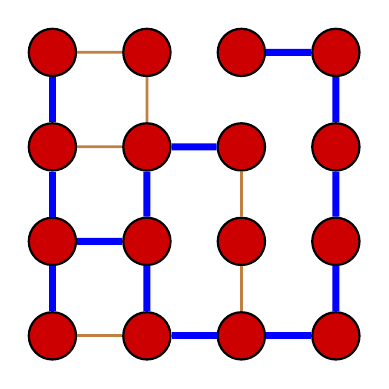
\begin{tikzpicture}[
            scale=1.2,
            node/.style={circle, draw=black, fill=red!80!black, thick, minimum size=0.6cm},
            regular_edge/.style={brown, line width=1pt},
            highlighted_edge/.style={blue, line width=2.5pt}
        ]

        % Create a 4x4 grid of nodes
        \foreach \i in {0,...,3} {
            \foreach \j in {0,...,3} {
                \node[node] (n\i\j) at (\i,\j) {};
            }
        }

        % Regular edges (brown)
        % Horizontal edges
        \draw[regular_edge] (n00) -- (n10);
        \draw[regular_edge] (n01) -- (n11);
        \draw[regular_edge] (n02) -- (n12);
        \draw[regular_edge] (n03) -- (n13);
        \draw[regular_edge] (n20) -- (n30);
        \draw[regular_edge] (n23) -- (n33);

        % Vertical edges
        \draw[regular_edge] (n10) -- (n11);
        \draw[regular_edge] (n11) -- (n12);
        \draw[regular_edge] (n12) -- (n13);
        \draw[regular_edge] (n20) -- (n21);
        \draw[regular_edge] (n21) -- (n22);
        \draw[regular_edge] (n30) -- (n31);
        \draw[regular_edge] (n31) -- (n32);
        \draw[regular_edge] (n32) -- (n33);

        % Highlighted edges (blue) - spanning tree
        % Horizontal edges
        \draw[highlighted_edge] (n12) -- (n22);
        \draw[highlighted_edge] (n01) -- (n11);
        \draw[highlighted_edge] (n10) -- (n20);
        \draw[highlighted_edge] (n20) -- (n30);
        \draw[highlighted_edge] (n23) -- (n33);

        % Vertical edges
        \draw[highlighted_edge] (n00) -- (n01);
        \draw[highlighted_edge] (n01) -- (n02);
        \draw[highlighted_edge] (n02) -- (n03);
        \draw[highlighted_edge] (n10) -- (n11);
        \draw[highlighted_edge] (n11) -- (n12);
        \draw[highlighted_edge] (n30) -- (n31);
        \draw[highlighted_edge] (n31) -- (n32);
        \draw[highlighted_edge] (n32) -- (n33);

        \end{tikzpicture}
        \caption{A spanning tree on a $4 \times 4$ grid graph. } 
        \label{fig:spanning_tree}
      \end{figure}
    \end{definition}

    Note that an unconnected graph will never have a spanning tree, but what about a connected graph? 

    \begin{theorem}[Spanning Trees of Connected Graphs]
      A connected graph will always have at least one spanning tree, not necessarily unique. 
    \end{theorem}

    Given a connected undirected weighted graph, we may want to find the \textbf{minimum spanning tree (MST)}, i.e. the spanning tree with edges $E^\prime$ such that the sum of the weights of all $e \in E^\prime$ is minimized.\footnote{An application of this is when we generally want to make sparse graphs. In a datacenter, wires can be expensive, so how I can minimize the length of wires to buy to construct a spanning subgraph?} How do we do this? There are two well-known algorithms to solve this. Prim's and Kruskal's algorithm.  
  
  \subsubsection{Prim's Algorithm with Cuts}

    Let's try to apply what we already know: Dijkstra. If we run Dijkstra on the graph starting at $s \in V$, we can get the shortest path from $s$ to every other node in the graph. This will give us a tree, but it may not be minimum. 

    \begin{figure}[H]
      \centering 
      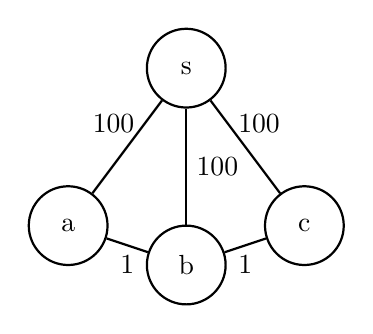
\begin{tikzpicture}[
          node/.style={circle, draw, minimum size=1cm, thick},
          edge/.style={-,thick}
      ]

      % Define node positions
      \node[node] (s) at (0,2) {s};
      \node[node] (a) at (-1.5,0) {a};
      \node[node] (b) at (0,-0.5) {b};
      \node[node] (c) at (1.5,0) {c};

      % Draw edges with weights
      \draw[edge] (s) -- node[left,near start] {100} (a);
      \draw[edge] (s) -- node[right] {100} (b);
      \draw[edge] (s) -- node[right,near start] {100} (c);
      \draw[edge] (a) -- node[below] {1} (b);
      \draw[edge] (b) -- node[below] {1} (c);

      \end{tikzpicture}
      \caption{If we run Dijkstra on $s$, then our output will be a tree of cost $300$, even when the actual MST can be of cost $102$ starting from $a$.} 
      \label{fig:dik_mst_prob}
    \end{figure}

    It may seem like this is just a problem of where we start, but even this is not the case. 

    \begin{figure}[H]
      \centering 
      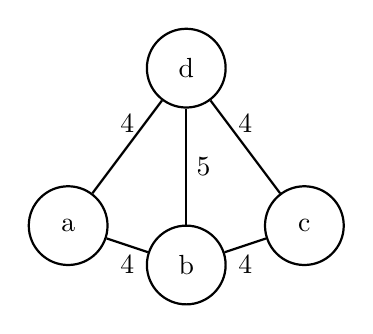
\begin{tikzpicture}[
          node/.style={circle, draw, minimum size=1cm, thick},
          edge/.style={-,thick}
      ]

      % Define node positions
      \node[node] (d) at (0,2) {d};
      \node[node] (a) at (-1.5,0) {a};
      \node[node] (b) at (0,-0.5) {b};
      \node[node] (c) at (1.5,0) {c};

      % Draw edges with weights
      \draw[edge] (d) -- node[left,near start] {4} (a);
      \draw[edge] (d) -- node[right] {5} (b);
      \draw[edge] (d) -- node[right,near start] {4} (c);
      \draw[edge] (a) -- node[below] {4} (b);
      \draw[edge] (b) -- node[below] {4} (c);

      \end{tikzpicture}
      \caption{No matter where we start from, we will never output the MST. The MST has cost $12$. If  we start from $b$ or $d$, we will get a tree of cost $13$. If we start from $a$ or $c$, we will get a tree of cost $16$.}
      \label{fig:dik_mst_prob2}
    \end{figure}

    \begin{definition}[Cuts]      
      Given graph $G(V, E)$, a \textbf{cut} is a partitioning of $V$ into $(S, V \setminus S)$. Furthermore, let $\mathrm{Cut}(S)$ be the number of edges with exactly one endpoint in $S$ and the other in $V \setminus S$. 
    \end{definition}

    \begin{theorem}[Cycles and Cuts]
      Given cycle $C \subset E$ in a graph and a cut $S \subset V$, 
      \begin{equation}
        | C \cap \mathrm{Cut}(S) | 
      \end{equation}
      is even. We can intuit this by visualizing the cycle as a long piece of looped string and a cut is a circle. The intersection between this circle and the string must be even since every time the cycle crosses through the cut, it must return back across the cut to the initial point.  
    \end{theorem}

    Now time for a bizarre theorem. 

    \begin{theorem}[Cut Property of MSTs]
      For all cuts $S \subset V$ of an undirected graph, the minimum cost edge in $\mathrm{Cut}(S)$ belongs to the MST. Furthermore, the converse is true: if we take all cuts and find all their minimum cost edges, these edges is precisely the MST! Therefore, an edge $e \in \mathrm{MST}$ iff $e$ is a min-cost edge for some cut. 

      \begin{figure}[H]
        \centering
        \begin{subfigure}[b]{0.48\textwidth}
        \centering
          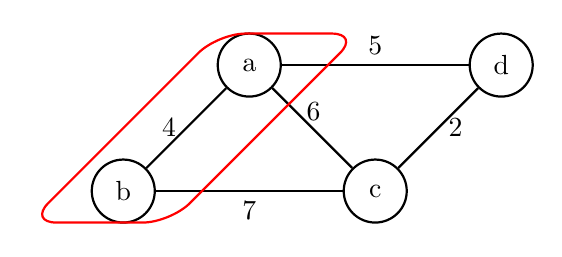
\begin{tikzpicture}[
            scale=0.8, 
            node/.style={circle, draw, minimum size=0.8cm, thick},
            edge/.style={-,thick},
            partition/.style={draw=red, thick}
          ]

          % Nodes with coordinates
          \node[node] (b) at (0,0) {b};
          \node[node] (c) at (4,0) {c};
          \node[node] (a) at (2,2) {a};
          \node[node] (d) at (6,2) {d};

          % Edges with weights
          \draw[edge] (a) -- node[above] {5} (d);
          \draw[edge] (a) -- node[left] {4} (b);
          \draw[edge] (a) -- node[right, pos=0.3] {6} (c);
          \draw[edge] (b) -- node[below] {7} (c);
          \draw[edge] (c) -- node[right] {2} (d);

          % Red partition boundary - left side partition as parallelogram
          % Using the same slope as the a-b edge and a-d edge
          \draw[partition, rounded corners=10pt] (-1.5,-0.5) -- (1.5,2.5) -- (3.75,2.5) -- (0.75,-0.5) -- cycle;

          \end{tikzpicture}
          \caption{}
        \end{subfigure}
        \hfill 
        \begin{subfigure}[b]{0.48\textwidth}
        \centering
          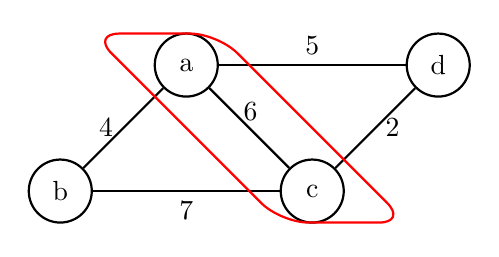
\begin{tikzpicture}[
            scale=0.8, 
            node/.style={circle, draw, minimum size=0.8cm, thick},
            edge/.style={-,thick},
            partition/.style={draw=red, thick}
          ]

          % Nodes with coordinates
          \node[node] (b) at (0,0) {b};
          \node[node] (c) at (4,0) {c};
          \node[node] (a) at (2,2) {a};
          \node[node] (d) at (6,2) {d};

          % Edges with weights
          \draw[edge] (a) -- node[above] {5} (d);
          \draw[edge] (a) -- node[left] {4} (b);
          \draw[edge] (a) -- node[right, pos=0.3] {6} (c);
          \draw[edge] (b) -- node[below] {7} (c);
          \draw[edge] (c) -- node[right] {2} (d);

          % Red partition boundary for right diagram
          \draw[partition, rounded corners=10pt] (3.5,-0.5) -- (0.5,2.5) -- (2.5,2.5) -- (5.5,-0.5) -- cycle;

          \end{tikzpicture}
          \caption{}
          \label{fig:}
        \end{subfigure}
        \label{fig:mst_cut_prop}
        \caption{In the left cut, the edges are $(a,d), (b, c), (a, c)$. The minimum weight is $5$ on the $(a, d)$ edge, so it must be in the MST. For the right cut, $(c, d)$ must be in the MST. }
      \end{figure}

      The final part is that if we have all edge costs different, then we will have a \textit{unique} MST. 
    \end{theorem}
    \begin{proof}
      We use a greedy approach and prove by contradiction. Suppose that this is not true, i.e. there exists a cut $S$ with minimum cost edge $e$, and $e \not\in \mathrm{MST}$. Then, there exists some other edge $e^\prime \in \mathrm{Cut}(S)$ that is in the MST, since the MST is spanning and it must cross over to connect the whole graph. Well if we just put $e$ in and take $e^\prime$ out, we will still have a spanning tree since it connects the left spanning tree to the right spanning tree, and we now have a cheaper tree. So the original cannot be the MST in the first place. 

      To prove the converse, consider some edge $e$ in the MST and we must prove that it is the minimum cost edge in some cut. Note that if we take $e$ out, then it divides the MST into two connected components, and we can just define the cut as these subsets of nodes. So this is in $\mathrm{Cut}(S)$ for some $S \subset V$. We can also prove that this is minimal since if it wasn't the minimum cost edge for some cut, we could have taken it out and inserted a cheaper edge $e^\prime$ to begin with, getting a cheaper spanning tree.   
    \end{proof}

    We can just brute force this logic into an algorithm by going through all possible cuts and adding the minimum cost edge to our MST set. It is clear that a cut is defined by a subset of $S$, so really the number of cuts a graph can have is $2^{|S| - 1}$, which is exponential in $n$. However, the minimum spanning tree isn't exponential since it must have $n-1$ edges, so there must be many cuts with the same minimum edge. 

    One way is to start with one vertex $a$ that contains the minimum cost edge $(a, b)$ across all edges.  This edge must be minimal and must be in the MST. Then we can look at the cut $S = \{a, b\}$ and look at that cut. We keep doing this, keeping track of the set of edges we need to look at after adding a new node to our cut. So the number of cuts I consider is equal to the number of edges in the spanning tree.

    \begin{algo}[Prim's Algorithm to Find MST]
      It turns out that we can modify Dijkstra to solve it. 
      \begin{algorithm}[H]
        \label{alg:prim}
        \begin{algorithmic}[1]
          \Require{Graph $G(E, V)$}

          \Function{Prim}{s}
            \State $S \gets \{s\}$  \Comment{Our initial cut}
            \State $\pi[v] \gets$ list of size $|V|$ of $+\infty$ \Comment{$\pi[u]$ is min cost of getting from $u$ into the $S$}
            \State $\pi[v] = w_{sv}$ for all $v \in V$ \Comment{initialize list with neighboring nodes from start $s$}

            \While{$S \neq V$}
              \State $u = \mathrm{argmin}_{v \notin S} \pi[v]$ \Comment{Find node having minimum cost to reach from $S$}
              \State $S \gets S \cup \{u\}$ \Comment{Adding this node to $S$ to expand our cut}
              \For{$u \not\in S$} \Comment{Since we expanded $S$, our min reach distances}
                \State $\pi[u] \gets \min\{\pi[u], w_{wu}\}$ \Comment{must be updated. It can only get shorter} 
              \EndFor \Comment{through a path from new $u$, so compare them}
            \EndWhile
            
          \EndFunction
        \end{algorithmic}
      \end{algorithm}

      \begin{figure}[H]
        \centering
        \begin{subfigure}[b]{0.48\textwidth}
        \centering
          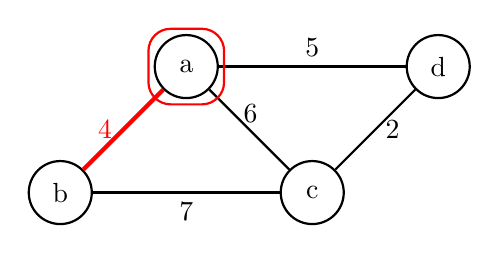
\begin{tikzpicture}[
            scale=0.8, 
            node/.style={circle, draw, minimum size=0.8cm, thick},
            edge/.style={-,thick},
            mstedge/.style={-,thick,red,line width=1.5pt},
            partition/.style={draw=red, thick}
          ]
          % Nodes with coordinates
          \node[node] (b) at (0,0) {b};
          \node[node] (c) at (4,0) {c};
          \node[node] (a) at (2,2) {a};
          \node[node] (d) at (6,2) {d};
          % Edges with weights
          \draw[edge] (a) -- node[above] {5} (d);
          \draw[mstedge] (a) -- node[left] {4} (b);
          \draw[edge] (a) -- node[right, pos=0.3] {6} (c);
          \draw[edge] (b) -- node[below] {7} (c);
          \draw[edge] (c) -- node[right] {2} (d);
          % Red partition boundary - around node a
          \draw[partition, rounded corners=8pt] (1.4,1.4) -- (2.6,1.4) -- (2.6,2.6) -- (1.4,2.6) -- cycle;
          \end{tikzpicture}
          \caption{}
        \end{subfigure}
        \hfill 
        \begin{subfigure}[b]{0.48\textwidth}
        \centering
          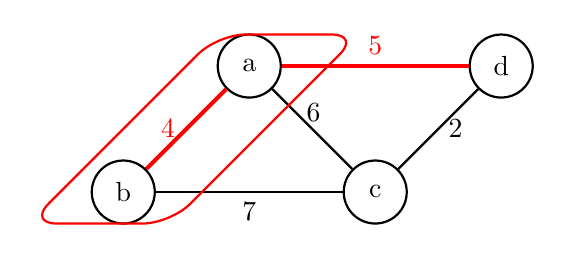
\begin{tikzpicture}[
            scale=0.8, 
            node/.style={circle, draw, minimum size=0.8cm, thick},
            edge/.style={-,thick},
            mstedge/.style={-,thick,red,line width=1.5pt},
            partition/.style={draw=red, thick}
          ]
          % Nodes with coordinates
          \node[node] (b) at (0,0) {b};
          \node[node] (c) at (4,0) {c};
          \node[node] (a) at (2,2) {a};
          \node[node] (d) at (6,2) {d};
          % Edges with weights
          \draw[mstedge] (a) -- node[above] {5} (d);
          \draw[mstedge] (a) -- node[left] {4} (b);
          \draw[edge] (a) -- node[right, pos=0.3] {6} (c);
          \draw[edge] (b) -- node[below] {7} (c);
          \draw[edge] (c) -- node[right] {2} (d);
          % Red partition boundary
          \draw[partition, rounded corners=10pt] (-1.5,-0.5) -- (1.5,2.5) -- (3.75,2.5) -- (0.75,-0.5) -- cycle;
          \end{tikzpicture}
          \caption{}
        \end{subfigure}
        
        \vspace{0.2cm}
        
        \begin{subfigure}[b]{0.48\textwidth}
        \centering
          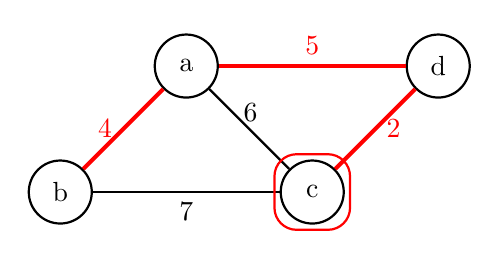
\begin{tikzpicture}[
            scale=0.8, 
            node/.style={circle, draw, minimum size=0.8cm, thick},
            edge/.style={-,thick},
            mstedge/.style={-,thick,red,line width=1.5pt},
            partition/.style={draw=red, thick}
          ]
          % Nodes with coordinates
          \node[node] (b) at (0,0) {b};
          \node[node] (c) at (4,0) {c};
          \node[node] (a) at (2,2) {a};
          \node[node] (d) at (6,2) {d};
          % Edges with weights
          \draw[mstedge] (a) -- node[above] {5} (d);
          \draw[mstedge] (a) -- node[left] {4} (b);
          \draw[edge] (a) -- node[right, pos=0.3] {6} (c);
          \draw[edge] (b) -- node[below] {7} (c);
          \draw[mstedge] (c) -- node[right] {2} (d);
          % Red partition boundary - around node c
          \draw[partition, rounded corners=8pt] (3.4,-0.6) -- (4.6,-0.6) -- (4.6,0.6) -- (3.4,0.6) -- cycle;
          \end{tikzpicture}
          \caption{}
        \end{subfigure}
        \caption{Step by step process of the method we mention above.}
        \label{fig:prim}
      \end{figure}
      
      We are really going through two loops. We add to the cut $S$ $n$ times and for each time we add, we must compute the argmin, which is also $O(n)$, so our total time complexity of $O(n^2)$.  
    \end{algo}

    However, this is not efficient, so we can introduce a minheap to get the argmin step faster. 

    \begin{algo}[Prim's Algorithm with MinHeap]
      \begin{algorithm}[H]
        \label{alg:prims}
        \begin{algorithmic}[1]
          \Require{Nodes $V$, Edges $E$}
          \Function{Prim}{V, E}
            \State mst $\gets$ [] \Comment{Initialize mst array to return}
            \State s $\gets$ 0 \Comment{Choose any starting node}
            \State visited $\gets$ set() \Comment{Our expanding set of cuts.}
            \State edges $\gets$ minheap() \Comment{The set of low-weight edges that we can explore from}
            \State add (weight, s, next\_node) for edges in E \Comment{Look for edges from s to expand our cut from.}

            \While{|visited| < |V|} \Comment{Until we have visited all cuts,}
              \State weight, frm, to $\gets$ pop from edges \Comment{Get the cheapest edge to explore}
              \If{to $\not\in$ visited} \Comment{If this isn't already in our cut, }
                \State add to $\rightarrow$ visited \Comment{Add it to our cut. From cut}
                \State add (frm, to, weight) to mst \Comment{property, this must be added to mst}

                \For{next\_to, next\_weight $\in$ E[to]} \Comment{After expanding, add newly discovered}
                  \If{next\_to $\not\in$ visited} \Comment{edges for future exploration}
                    \State push (next\_weight, to, next\_to) to edges
                  \EndIf
                \EndFor
              \EndIf
            \EndWhile 

            \State \Return{mst} \Comment{of form (from, to, weight)}
          \EndFunction
        \end{algorithmic}
      \end{algorithm}

      You essentially push $n$ times and pop $m$ times, and the time per push and pop is $\log_2 (n)$. Therefore, the total time to push is $n \log(n)$ and to pop is $m \log (n)$, making the total runtime $O((n + m) log(n)) = O(m \log{n})$. 
    \end{algo}

    This can be sped up even faster if we use Fibonacci heaps or assume extra structure on the graph. 

  \subsubsection{Kruskal's Algorithm}

    If we were to try and construct this algorithm from scratch, we may take a greedy approach by incrementally adding the minimum cost edge from your cut. However, there is one thing to check: have we entered a cycle? Checking whether the next added node $a$ completes a cycle in $S \cup \{a\}$ is nontrivial. 

    \begin{theorem}[Cycle Property]
      For all cycles $C$, the max cost edge of $C$ does not belong to MST. 
    \end{theorem}

    Therefore, you can take $S$ and either add to it using the cut property or delete candidates from it using the cycle property. What is the best order to do this in? Kruskal's algorithm answers this question, which takes a greedy approach. 

    \begin{algo}[General Kruskal's Algorithm]
      The general idea is that we sort $e \in E$ in increasing cost, and for each $e \in E$, we use either the cut or cycle property to decide whether $e$ goes in or out. 

      \begin{algorithm}[H]
        \label{alg:prim_kruskal}
        \begin{algorithmic}[1]
          \Require{Graph $G(V, E)$}
          \Function{Kruskal}{V, E}
            \State sort $E$ in increasing cost 
            \State $T \gets \{\}$
            \For{$e \in E$}
              \If{$T \cup \{e\}$ does not have cycle} 
                \State $T \gets T \cup \{e\}$ \Comment{Cut property}
              \Else \Comment{Cycle property} 
                \State continue \Comment{discard $e$ since from sorting, this edge is heaviest in cycle}
              \EndIf
            \EndFor
          \EndFunction
        \end{algorithmic}
      \end{algorithm}

      \begin{figure}[H]
        \centering
        \begin{subfigure}[b]{0.48\textwidth}
        \centering
          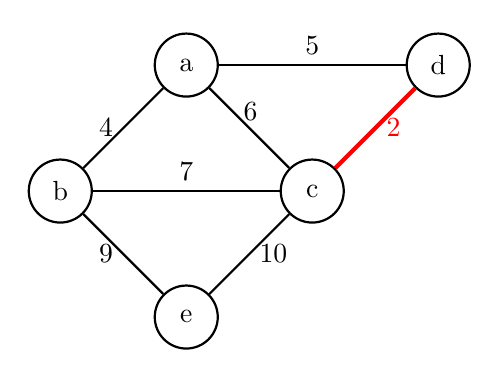
\begin{tikzpicture}[
            scale=0.8, 
            node/.style={circle, draw, minimum size=0.8cm, thick},
            edge/.style={-,thick},
            mstedge/.style={-,thick,red,line width=1.5pt}
          ]
          % Nodes with coordinates
          \node[node] (b) at (0,0) {b};
          \node[node] (c) at (4,0) {c};
          \node[node] (a) at (2,2) {a};
          \node[node] (d) at (6,2) {d};
          \node[node] (e) at (2,-2) {e};
          
          % Edges with weights
          \draw[edge] (a) -- node[above] {5} (d);
          \draw[edge] (a) -- node[left] {4} (b);
          \draw[edge] (a) -- node[right, pos=0.3] {6} (c);
          \draw[edge] (b) -- node[above] {7} (c);
          \draw[mstedge] (c) -- node[right] {2} (d);
          \draw[edge] (b) -- node[left] {9} (e);
          \draw[edge] (c) -- node[right] {10} (e);
          \end{tikzpicture}
          \caption{}
        \end{subfigure}
        \hfill 
        \begin{subfigure}[b]{0.48\textwidth}
        \centering
          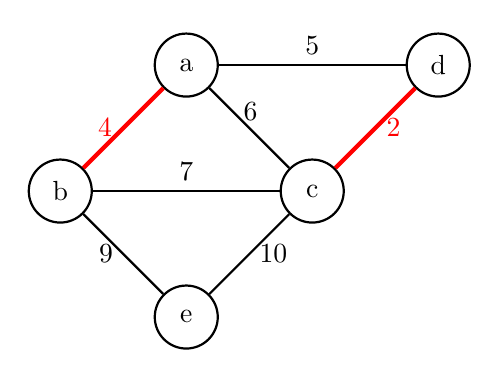
\begin{tikzpicture}[
            scale=0.8, 
            node/.style={circle, draw, minimum size=0.8cm, thick},
            edge/.style={-,thick},
            mstedge/.style={-,thick,red,line width=1.5pt}
          ]
          % Nodes with coordinates
          \node[node] (b) at (0,0) {b};
          \node[node] (c) at (4,0) {c};
          \node[node] (a) at (2,2) {a};
          \node[node] (d) at (6,2) {d};
          \node[node] (e) at (2,-2) {e};
          
          % Edges with weights
          \draw[edge] (a) -- node[above] {5} (d);
          \draw[mstedge] (a) -- node[left] {4} (b);
          \draw[edge] (a) -- node[right, pos=0.3] {6} (c);
          \draw[edge] (b) -- node[above] {7} (c);
          \draw[mstedge] (c) -- node[right] {2} (d);
          \draw[edge] (b) -- node[left] {9} (e);
          \draw[edge] (c) -- node[right] {10} (e);
          \end{tikzpicture}
          \caption{}
        \end{subfigure}
        
        \vspace{0.5cm}
        
        \begin{subfigure}[b]{0.48\textwidth}
        \centering
          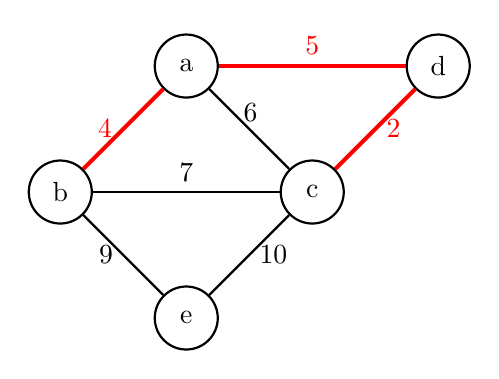
\begin{tikzpicture}[
            scale=0.8, 
            node/.style={circle, draw, minimum size=0.8cm, thick},
            edge/.style={-,thick},
            mstedge/.style={-,thick,red,line width=1.5pt}
          ]
          % Nodes with coordinates
          \node[node] (b) at (0,0) {b};
          \node[node] (c) at (4,0) {c};
          \node[node] (a) at (2,2) {a};
          \node[node] (d) at (6,2) {d};
          \node[node] (e) at (2,-2) {e};
          
          % Edges with weights
          \draw[mstedge] (a) -- node[above] {5} (d);
          \draw[mstedge] (a) -- node[left] {4} (b);
          \draw[edge] (a) -- node[right, pos=0.3] {6} (c);
          \draw[edge] (b) -- node[above] {7} (c);
          \draw[mstedge] (c) -- node[right] {2} (d);
          \draw[edge] (b) -- node[left] {9} (e);
          \draw[edge] (c) -- node[right] {10} (e);
          \end{tikzpicture}
          \caption{}
        \end{subfigure}
        \hfill
        \begin{subfigure}[b]{0.48\textwidth}
        \centering
          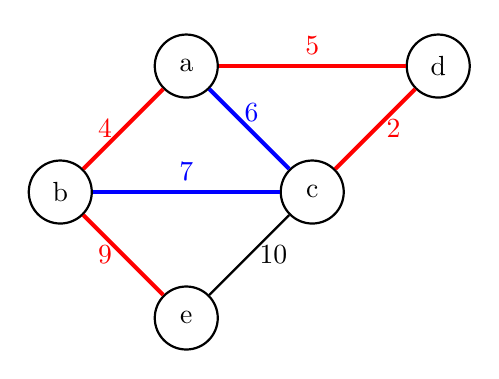
\begin{tikzpicture}[
            scale=0.8, 
            node/.style={circle, draw, minimum size=0.8cm, thick},
            edge/.style={-,thick},
            mstedge/.style={-,thick,red,line width=1.5pt},
            blueedge/.style={-,thick,blue,line width=1.5pt}
          ]
          % Nodes with coordinates
          \node[node] (b) at (0,0) {b};
          \node[node] (c) at (4,0) {c};
          \node[node] (a) at (2,2) {a};
          \node[node] (d) at (6,2) {d};
          \node[node] (e) at (2,-2) {e};
          
          % Edges with weights
          \draw[mstedge] (a) -- node[above] {5} (d);
          \draw[mstedge] (a) -- node[left] {4} (b);
          \draw[blueedge] (a) -- node[right, pos=0.3] {6} (c);
          \draw[blueedge] (b) -- node[above] {7} (c);
          \draw[mstedge] (c) -- node[right] {2} (d);
          \draw[mstedge] (b) -- node[left] {9} (e);
          \draw[edge] (c) -- node[right] {10} (e);
          \end{tikzpicture}
          \caption{}
        \end{subfigure}
        \caption{Kruskal's algorithm. In the last step, we see that the next minimum cost edge of 6 and 7 forms a cycle, so we add the edge of length 9.}
        \label{fig:kruskal}
      \end{figure}

      The sorting of edges take $O(m \log{m})$ time, and after sorting, we iterate through all the edges and apply $m$ find-union algorithm, which each take at most $O(\log{n})$ time. Therefore, the overall complexity is $O(m \log{m} + m \log{n})$. However, the value of $m$ can be at most $O(n^2)$, so the two logarithms are essentially the same, arriving at the final runtime of $O(m \log{n})$. 
    \end{algo}

    The way to prove that this is correct is to show that every step you do is correct, known as \textit{structural induction}, either because of one of the two properties. Say that so far, we have some edges in $V$ which forms a partition of $V = \sqcup_i T_i$ of disjoint trees (can be trees, one edge, or just single nodes). We are looking at the next biggest edge $e = (a, b)$. There are two possibilities. 
    \begin{enumerate}
      \item If $a, b$ are both in a single $T_i$, then this forms a cycle and can be thrown away since this is the max cost edge in the cycle by the cycle property. 
      \item If $a, b$ connect $T_i$ and $T_j$ for $i \neq j$, then this edge is in $\mathrm{Cut}(T_i)$ and is the minimum cost edge since the rest of the edges in $\mathrm{Cut}(T_i)$ come next in the sorted $E$. Therefore this must be included by the cut property. 
    \end{enumerate}


    \begin{figure}[H]
      \centering 
      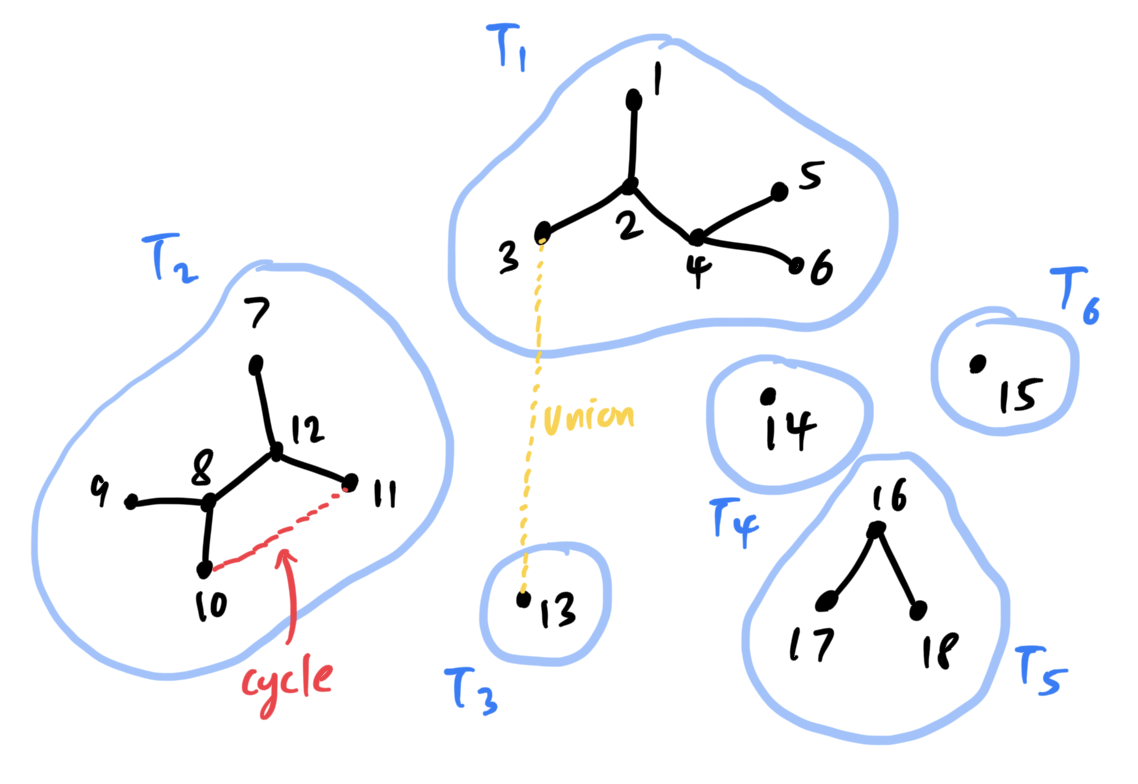
\includegraphics[scale=0.4]{img/sets.png}
      \caption{Each $T_i$ is a component formed by the edges chosen so far. For example, $T_1 = \{1, 2, 3, 4, 5, 6\}, \ldots$. We can either discard an edge (red) or include an edge (yellow). } 
      \label{fig:sets}
    \end{figure}

    The only bottleneck in here is line 5, where we check if $e$ does not complete a cycle in $T$. It will obviously not be efficient to do BFS, construct a tree, and see if there is a loop by checking if two points in the same layer are connected. It may help to decompose this algorithm into two steps: what is being stored and what is being checked? 

    Note that from our visual, we are really just keeping a set of these points that each make a subtree and connecting them together. How do we efficiently search for which cluster a point is a part of and efficiently merge two clusters? We could use a hashmap but this wouldn't work. We need something like a doubly linked list. 

    \begin{algo}[Kruskal's Algorithm]
      The implementation uses the Union-Find data structure. For clarity, we will not elaborate it but will show the full pseudocode. 
      \begin{algorithm}[H]
        \label{alg:kruskal}
        \begin{algorithmic}
          \Require{Nodes V. Edges $E = \{(u, v, w)\}$ where $u, v \in V$ and $w > 0$ is a weight. }
          \State 
          \Function{Kruskal}{V, E}
            \State $n \gets |V|$ 
            \State sort $E$ in increasing order of weights. \Comment{Needed for Kruskal}
            \State parent $\gets [0, \ldots, n-1]$ \Comment{Initialize the disjoint cluster each node is in}
            \State rank $\gets$ list of $0$s of size $n$ 

            \Function{Find}{x} 
              \If{parent[x] $\neq$ x} 
              \State parent[x] $\gets$ Find(parent[x]) \Comment{Path compression}
              \EndIf
              \State \Return{parent[x]}
            \EndFunction

            \Function{Union}{x, y} 
              \State px, py = find(x), find(y) 
              \If{px = py} 
                \State \Return{False}
              \EndIf
              \If{rank[px] < rank[py]} 
                \State parent[px] $\gets$ py
              \ElsIf{rank[px] > rank[py]}
                \State parent[py] $\gets$ px
              \Else{}
                \State parent[py] $\gets$ px 
                \State rank[px] $\gets$ rank[px] + 1
              \EndIf
              \State \Return{True}
            \EndFunction

            \State mst $\gets$ [] 
            \For{u, v, weight $\in$ edges} 
              \If{union(u, v)} 
                \State add (u, v, weight) to mst
              \EndIf 
              \If{len(mst) = n - 1}
                \State break
              \EndIf 
            \EndFor

            \State \Return{mst}
          \EndFunction
        \end{algorithmic}
      \end{algorithm}
    \end{algo}
    
    To analyze the runtime of this, we define the function. 

    \begin{definition}[Ackerman Function]
      The \textbf{Ackerman function} is one of the fastest growing functions known. It is practically infinity. 
      \begin{equation}
        A(m,n) = 
        \begin{cases} 
          n+1 & \text{if } m = 0 \\
          A(m-1,1) & \text{if } m > 0 \text{ and } n = 0 \\
          A(m-1,A(m,n-1)) & \text{if } m > 0 \text{ and } n > 0
        \end{cases} 
      \end{equation}
      The inverse Ackerman function therefore grows extremely slowly. 
    \end{definition}

    If we optimize the steps in Kruskal's algorithm, we can get its runtime to 
    \begin{equation}
      O((m + n) \log^{\ast} (n))
    \end{equation}
    which is practically linear. 

  \subsubsection{Applications}

    Here is a way to cluster data, a surprising way to apply MSTs. It is the most widely used application, especially in data science. The problem is that given $n$ data points $x_i \in \mathbb{R}^d$ and an integer $k$, we want to partition the points into $k$ groups $\mathbf{C} = (C_1, \ldots, C_k)$ where $\mathbf{x} = \sqcup_i C_i$. You want to distances between the points within a group to be small and the distances between groups to be large. We can think of finding the objective which takes every pair of clusters and computes the minimum distance between these clusters, and we want to maximize this distance over all pairs of clusters.  

    \begin{algo}[Single Linkage/Hierarchical Clustering]
      The general idea is to take this dense graph, find the MST, and cut off the largest edges from this MST, which will give you $k$ components. This is the answer. Or really, you can use Kruskal's algorithm and terminate earlier when $T$ has $k$ sets/components. 
      Note that as we add edges as we construct our MST, we are merging two clusters into one. So that all you are doing is finding the next pair of closest points and merging the clusters that they are a part of. 

      \begin{algorithm}[H]
        \label{alg:clustering}
        \begin{algorithmic}[1]
          \Require{Nodes $V = \{v_i\} \subset \mathbb{R}^n$}
          \Function{Cluster}{V}
            \State Run Kruskal and at each iteration, check if you have $K$ clusters. 
            \State If so, terminate and return the \texttt{parent} list. 
          \EndFunction
        \end{algorithmic}
      \end{algorithm}
    \end{algo}

    \begin{theorem}
      The algorithm above minimizes the objective function. 
      \begin{equation}
        \argmax_{\mathbf{C}} \min_{p \in C_i, q \in C_j} \{ d(p, q) \}
      \end{equation}
    \end{theorem}
    \begin{proof}
      Let $\mathbf{C}^\ast$ be the MST clustering. We claim that for any other clustering $\mathbf{C} = \{C_1, \ldots, C_k\}$,  
      \begin{equation}
        \mathrm{min dist}(\mathbf{C}) \leq \mathrm{min dist}(\mathbf{C}^{\ast})
      \end{equation}
      Assume that this was not the case, so $\mathrm{min dist}(\mathbf{C}) > \mathrm{min dist}(\mathbf{C}^{\ast})$ and therefore there exists a $p, q \in C_i, C_j$ such that $d(p, q) = \mathrm{mindist}(\mathbf{C}) > \mathrm{min dist}(\mathbf{C}^\ast)$. Since this is a different clustering, $p, q$ must have been in the same cluster $C_i^\ast$. But note that since Kruskal adds edges in increasing length, all edges within a cluster must have length less edges that go across two clusters. 

      \begin{figure}[H]
        \centering 
        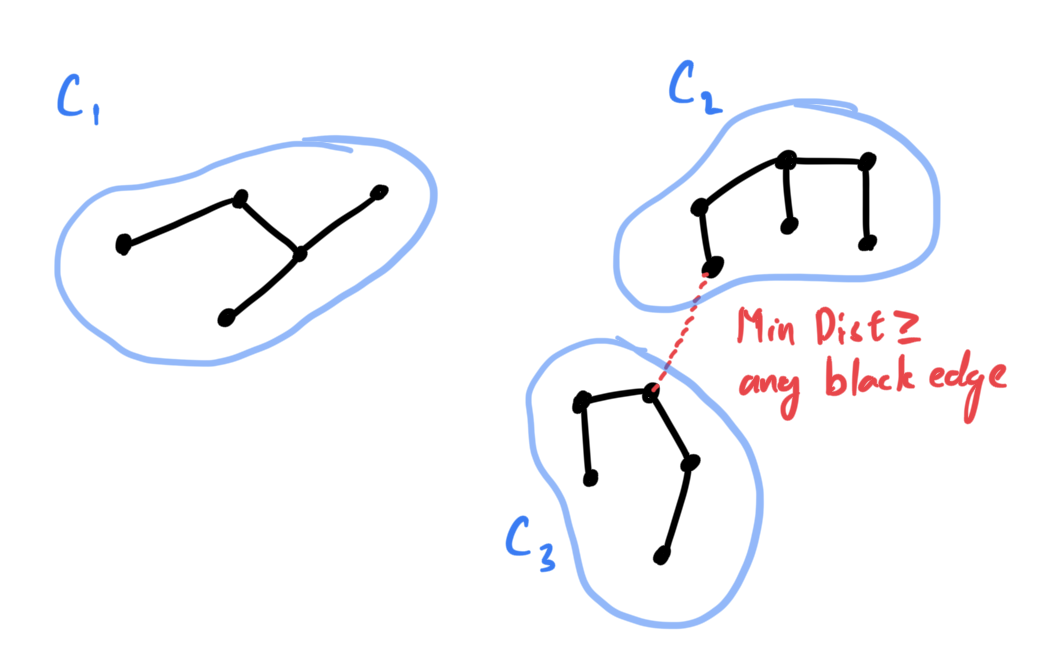
\includegraphics[scale=0.4]{img/mindist.png}
        \label{fig:mindist}
      \end{figure}

      So $d(p, q)$ must be the less than the length of all edges within a cluster in $\mathbf{C}^\ast$. But all within-cluster edges must be smaller than $\mathrm{min dist}(\mathbf{C}^\ast)$, meaning that $\mathrm{min dist}(\mathbf{C}^\ast) > d(p, q)$, contradicting the fact that is is greater, and we are done. 
    \end{proof}

    If you define the distance between two clusters to be the distance between the centroids (mean point), then this is called \textit{average linkage} (min avg distance). If we define the cluster distance as the maximum distance between two points, then it is called \textit{complete linkage} (min max distance). Kruskal's algorithm only worked for the single linkage case but may not work for these additional definitions. This is why there is usually a whole suite of clustering algorithms for a particular problem and we just find out which one fits the data the best. Furthermore, we have done \textit{bottom-up clustering}, where we took individual points to make clusters. In \textit{top-down clustering}, we take the whole set and cut it up into clusters.  

